% Format teze zasnovan je na paketu memoir
% http://tug.ctan.org/macros/latex/contrib/memoir/memman.pdf ili
% http://texdoc.net/texmf-dist/doc/latex/memoir/memman.pdf
% 
% Prilikom zadavanja klase memoir, navedenim opcijama se podešava 
% veličina slova (12pt) i jednostrano štampanje (oneside).
% Ove parametre možete menjati samo ako pravite nezvanične verzije
% mastera za privatnu upotrebu (na primer, u b5 varijanti ima smisla 
% smanjiti 
\documentclass[12pt,oneside]{memoir} 

% da bi se u sadrzaju video subsection
\setcounter{tocdepth}{3}
\setsecnumdepth{subsubsection}

% definicije
\newtheorem{definition}{Definicija}

%find i copy/paste
\usepackage{cmap}

\usepackage{caption}
\usepackage{subcaption}

\usepackage{listings}

\usepackage{amsmath}
\usepackage{hyperref}
% razmak medju paragrafima
\setlength{\parskip}{1em}

% linkovi u sadržaju
\usepackage{hyperref}
\usepackage{url}
\hypersetup{
    colorlinks,
    citecolor=blue,
    filecolor=black,
    linkcolor=blue,
    urlcolor=black
}

% Paket koji definiše sve specifičnosti master rada Matematičkog fakulteta
\usepackage[latinica]{matfmaster} 

%bibliografija
\bib{rad}

%
% Podrazumevano pismo je ćirilica.
%   Ako koristite pdflatex, a ne xetex, sav latinički tekst na srpskom jeziku
%   treba biti okružen sa \lat{...} ili \begin{latinica}...\end{latinica}.
%
% Opicija [latinica]:
%   ako želite da pišete latiniciom, dodajte opciju "latinica" tj.
%   prethodni paket uključite pomoću: \usepackage[latinica]{matfmaster}.
%   Ako koristite pdflatex, a ne xetex, sav ćirilički tekst treba biti
%   okružen sa \cir{...} ili \begin{cirilica}...\end{cirilica}.
%
% Opcija [biblatex]:
%   ako želite da koristite reference na više jezika i umesto paketa
%   bibtex da koristite BibLaTeX/Biber, dodajte opciju "biblatex" tj.
%   prethodni paket uključite pomoću: \usepackage[biblatex]{matfmaster}
%
% Opcija [b5paper]:
%   ako želite da napravite verziju teze u manjem (b5) formatu, navedite
%   opciju "b5paper", tj. prethodni paket uključite pomoću: 
%   \usepackage[b5paper]{matfmaster}. Tada ima smisla razmisliti o promeni
%   veličine slova (izmenom opcije 12pt na 11pt u \documentclass{memoir}).
%
% Naravno, opcije je moguće kombinovati.
% Npr. \usepackage[b5paper,biblatex]{matfmaster}

% Pomoćni paket koji generiše nasumičan tekst u kojem se javljaju sva slova
% azbuke (nema potrebe koristiti ovo u pravim disertacijama)
\usepackage[latinica]{}%{pangrami}

% Datoteka sa literaturom u BibTex tj. BibLaTeX/Biber formatu
%\bib{matfmaster-primer}

% Ime kandidata na srpskom jeziku (u odabranom pismu)
\autor{Nikola Z. Vidič}
% Naslov teze na srpskom jeziku (u odabranom pismu)
\naslov{Primena mašinskog učenja u verifikaciji softvera}
% Godina u kojoj je teza predana komisiji
\godina{2018}
% Ime i afilijacija mentora (u odabranom pismu)
\mentor{dr Milena \textsc{Vujošević Janičić}, docent\\ Univerzitet u Beogradu, Matematički fakultet}
% Ime i afilijacija prvog člana komisije (u odabranom pismu)
\komisijaA{dr Mladen \textsc{Nikolić}, docent\\ Univerzitet u Beogradu, Matematički fakultet}
% Ime i afilijacija drugog člana komisije (u odabranom pismu)
\komisijaB{dr Filip \textsc{Marić}, vanredni profesor\\ Univerzitet u Beogradu, Matematički fakultet}
% Ime i afilijacija trećeg člana komisije (opciono)
% \komisijaC{}
% Ime i afilijacija četvrtog člana komisije (opciono)
% \komisijaD{}
% Datum odbrane (odkomentarisati narednu liniju i upisati datum odbrane ako je poznat)
% \datumodbrane{}

% Apstrakt na srpskom jeziku (u odabranom pismu)

\apstr{%
%\pangrami
}

% Ključne reči na srpskom jeziku (u odabranom pismu)
\kljucnereci{}%analiza, geometrija, algebra, logika, računarstvo, astronomija}

\begin{document}
% ==============================================================================
% Uvodni deo teze
\frontmatter
% ==============================================================================
% Naslovna strana
\naslovna
% Strana sa podacima o mentoru i članovima komisije
\komisija
% Strana sa posvetom (u odabranom pismu)
\posveta{}%Mami, tati i dedi}
% Strana sa podacima o disertaciji na srpskom jeziku
\apstrakt
% Sadržaj teze
\tableofcontents*

% ==============================================================================
% Glavni deo teze
\mainmatter
% ==============================================================================

% ------------------------------------------------------------------------------
\chapter{Uvod}
% ------------------------------------------------------------------------------
%\pangrami




\chapter{Mašinsko učenje}
\label{chp:mašinsko učenje}

%Termin \textit{mašinsko učenje (eng. machine learning)} nastaje 1959-te godine, a njegov tvorac je Artur Semjuel (Arthur Samuel) američki pionir u poljima kompjuterskih igara i \textit{veštačke inteligencije (eng. artificial intelligence)}. 
%Sama ideja mašinskog učenja javlja se još ranije, u radovima Alena Tjuringa (Alan Turing) četrdesetih godina dvadesetog veka. %Mašinsko učenje nastaje iz potrage za veštačkom inteligencijom. 
%Razvoj mašinskog učenja vođen je željom da se razume i oponaša ljudski potencijal za učenje. 
%Ubrzo nakon što veštačka inteligencija postaje univerzitetska disciplina pojavljuju se naučnici zainteresovani da vide kako mašine uče na osnovu podataka. Prvi pokušaji takvog načina učenja bili su u vidu \textit{neuronskih mreža (eng. neural networks)} koje su pedesetih godina najčešće imale formu \textit{perceptrona (eng. perceptron)}. 

Sama ideja \textit{mašinskog učenja (eng.~machine learning)} javlja se još četrdesetih godina dvadesetog veka u radovima Alana Tjuringa (Alan Turing). Razvoj mašinskog učenja vođen je željom da se razume i oponaša ljudski potencijal za učenje. Pedesetih godina mašinsko učenje se razvija zajedno sa pojmom perceptrona, pretka neuronskih mreža. %Razvoj mašinskog učenja u formi neuronskih mreža nastavlja se sve do devedesetih godina.
Razvoj mašinskog učenja u formi neuronskih mreža nastavlja se, uz uspone i padove interesovanja, sve do danas. Početkom dvehiljaditih dešava se proboj na polju razvoja \textit{veštačke inteligencije (eng.~artificial inteligence)} i mnogi problemi za koje se smatralo da će jos dugo ostati nerešeni bivaju rešeni, velikim delom zahvaljujući mašinskom učenju. Uopšteno, ,,mašinsko učenje predstavlja disciplinu koja se bavi konstrukcijom sistema koji se prilagođavaju i popravljaju svoje performanse sa povećanjem iskustva, oličenog u količini relevantnih podataka \cite{mladen}''. Mašinsko učenje proučava indukcijski način zaključivanja tj. generalizaciju (uopštavanje ka univerzalnim zaključcima). Primene mašinskog učenja su brojne: prepoznavanje različitih oblika na slikama (na primer, lica i tumora), autonomno upravljanje vozilima (na primer, automobilima ili letelicama), igranje igara na tabli kao što je šah, klasifikacija teksta, prepoznavanje cifara i mnoge druge \cite{mladen}.

Mašinsko učenje za rešavanje problema koristi različite metode. Ove metode se prema prirodi problema učenja svrstavaju u jednu od tri grupe: \textit{nadgledano učenje} (eng.~\textit{supervised learning}), \textit{nenadgledano učenje} (eng.~\textit{unsupervised learning}) ili \textit{učenje potkrepljivanjem} (eng.~\textit{reinforcement learning}). U nastavku teksta detaljnije su opisane neke tehnike nadgledanog učenja. Detaljnije informacije o nenadgledanom učenju i o učenju potkrepljivanjem nisu potrebne za razumevanje teze i mogu se naći u literaturi \cite{mlm, reinforcement-learning, mladen}.

\section{Nadgledano učenje}
Nadgledano učenje se odlikuje datim vrednostima ulaza, ali i datim vrednostima izlaza koji im odgovaraju. Na osnovu tih podataka potrebno je odrediti vezu koja postoji između ulaza i izlaza.% tj. podacima na osnovu kojih se uči i izlaznim podacima tj. podacima koje je potrebno naučiti. 
%Understanding Machine Learning: From Theory to Algorithms
Nadgledano učenje se može posmatrati kao vid učenja u kom se znanje stiče iskustvom. Iskustvo je sadržano u podacima za treniranje, a stečeno znanje se primenjuje na nove podatke. 
%
Naziv je posledica sličnosti postupka nadgledanog učenja i učenja u kome profesor zada učeniku zadatke i nakon što ih učenik reši, d\^a učeniku odgovore radi poređenja rezultata. Algoritmi mašinskog učenja se opisuju kao učenje ciljne funkcije \textit{f} koja najbolje opisuje vezu između ulaznih promenljivih \textit{x} i izlazne promenljive \textit{y}, odnosno $y=f(x)$. Naučena veza (ciljna funkcija $f$) se kasnije koristi za buduća predviđanja izlaza $y$ na osnovu novih vrednosti ulaza $x$. Najčešće je ulaz predstavljen vektorom vrednosti promenljivih koje se nazivaju \textit{atributima} (eng.~\textit{features}), a izlaz kao jedna promenljiva koja se zove \textit{ciljna promenljiva} (eng.~\textit{target variable}). 
Kako se u današnje vreme raspolaže ogromnim količinama podataka merenim gigabajtima i terabajtima, neophodno je pronaći metode koje automatski pronalaze veze između promenljivih. Veze tj. izgrađene ciljne funkcije se nazivaju \textit{modelima mašinskog učenja}. Postoji veliki broj modela i ne opisuju svi podjednako dobro veze među podacima. Od kvalitetnog modela se očekuje da vrši dobru generalizaciju tj. da prilikom predviđanja retko greši \cite{mladen, mlm, UMLFTA}. %https://machinelearningmastery.com/how-machine-learning-algorithms-work/

Osnovne vrste nadgledanog učenja su \textit{klasifikacija} i \textit{regresija}.
,,Klasifikacija je problem predviđanja kategoričke ciljne promenljive \cite{mladen}''. Vrednosti kategoričke promenljive pripadaju nekom konačnom skupu, pri čemu ne postoji uređenje među tim vrednostima. 
,,Regresija je problem predviđanja neprekidne ciljne promenljive \cite{mladen}''.  Neprekidne promenljive uzimaju vrednosti iz neograničenog skupa vrednosti.

\begin{description}
\item[Preprilagođavanje modela] Model klasifikacije može imati dve vrste grešaka: greške u fazi treniranja i greške u generalizaciji. Greška u fazi treniranja modela predstavlja broj grešaka usled pogrešne klasifikacije trening instanci. Greška u generalizaciji predstavljaju očekivanu grešku koju model pravi prilikom određivanja klasa nepoznatih instanci. Odlike dobrog modela su prilagodljivost trening podacima i tačno predviđanje klasa novih instanci. To znači da dobri modeli imaju male vrednosti grešaka i u fazi treniranja i u fazi generalizacije. Model koji previše dobro odgovara trening podacima, odnosno ima malu grešku u fazi treniranja, može imati veću grešku u generalizaciji u odnosu na model sa većom greškom u fazi treniranja. Takva situacija se naziva \textit{preprilagođavanje modela} (eng.~model overfitting). Preprilagođavanje može nastati: (1) zbog nedostatka reprezentativnih uzoraka - model će doći do pogrešnih zaključaka zbog nedovoljnog broja trening podataka. (2) kao posledica prisustva šuma (eng.~noise) među trening podacima. Na primer, nova instanca će biti pogrešno klasifikovana zato što su vrednosti nekih njenih atributa identične vrednostima atributa pogrešno klasifikovane trening instance.  (3) kod modela čiji algoritmi učenja primenjuju proceduru višestrukog poređenja (eng.~multiple comparison procedure). Neka je $T_0$ inicijalno drvo odlučivanja a $T_x$ drvo nakon što se u njega doda unutrašnji čvor za atribut $x$. %Čvor se može dodati u stablo ako je dobit $\Delta(T_0, T_x)$ veća od nekog zadatog parametra $\alpha$. Ako postoji samo jedan uslov testiranja atributa izbor dovoljno velike vrednosti parametra $\alpha$ eliminiše dodavanje lažno najboljih čvorova podele (eng.~spurious nodes) u stablo. Realnost je da u praksi postoji više uslova testiranja atributa, a drvo odlučivanja treba da izabere najbolji atribut podele $x_k$ iz skupa atributa \{$x_1, x_2,...,x_k$\} testiranjem uslova $\Delta(T_0, T_{x_{max}})>\alpha$. Sa većim brojem atributa za razmatranje raste i verovatnoća da će se pronaći atribut koji zadovoljava uslov $\Delta(T_0, T_{x_{max}})>\alpha$. %U ovoj situaciji algoritam može nenamerno da dodaje lažno najbolje čvorove podele, što vodi preprilagođavanju modela. 
%Ne moraju nužno svi atributi završiti kao čvorovi stabla odlučivanja da bi ono bilo dobar model. 
%Stablo dobijeno dodavanjem novog čvora nije obavezno i bolje stablo tj. bolji model. 
Dodavanjem novog čvora ne dobija se obavezno bolje drvo tj. bolji model. Čvor se može dodati u stablo ako je dobit $\Delta(T_0, T_x)$ veća od nekog zadatog parametra $\alpha$. Ovaj način dodavanja čvorova u stablo je zavisan od funkcije podele $\Delta$ i parametra $\alpha$. Ako postoji samo jedan uslov testiranja atributa izbor dovoljno velike vrednosti parametra $\alpha$ eliminiše dodavanje ,,podmetnutih'' čvorova (eng.~spurious nodes) u stablo. Podmetnuti čvorovi zadovoljavaju uslov $\Delta(T_0, T_{x_{max}})>\alpha$ ali se njihovim dodavanjem ne dobija bolji model. Realnost je da u praksi postoji više uslova testiranja atributa, a drvo odlučivanja treba da izabere najbolji atribut podele $x_k$ iz skupa atributa \{$x_1, x_2,...,x_k$\} testiranjem uslova $\Delta(T_0, T_{x_{max}})>\alpha$. Sa većim brojem atributa za razmatranje raste i verovatnoća da će se pronaći atribut koji zadovoljava uslov $\Delta(T_0, T_{x_{max}})>\alpha$. U ovoj situaciji algoritam može da dodaje ,,podmetnute'' čvorove podele, što vodi preprilagođavanju modela. Zato treba modifikovati funkciju dobiti $\Delta$ ili parametar $\alpha$ tako da u obzir uzimaju $k$  \cite{mitic}.
\end{description}

U nastavku će detaljnije biti opisani modeli klasifikacije zasnovani na algoritmima \textit{k} najbližih suseda, 
slučajnim šumama i logističkoj regresiji.

%% kNN
\subsection{Algoritam \textit{k} najbližih suseda}

Klasifikatori zasnovani na algoritmu \textit{k} najbližih suseda spadaju u klasifikatore zasnovane na instancama. Kod klasifikatora zasnovnih na instancama faza treniranja se odlaže sve do poslednjeg koraka procesa klasifikacije. Za takve klasifikatore se kaže da ,,lenjo'' uče (eng.~lazy learners). Najjednostavniji opis logike učenja zasnovanog na instancama je da slične instance imaju slične oznake klasa (,,ako hoda kao patka, priča kao patka i izgleda kao patka, onda je najverovatnije patka \cite{mitic}'') \cite{aggarwal}.

Reprezentacija modela koji koriste algoritam $k$ najbližih suseda je čitav skup trening podataka. Pošto nema eksplicitnog modela, nema ni potrebe za učenjem istog. Trening podaci se skladište u memoriji pa je poželjno njihovo redovno održavanje (ažuriranje kada se dođe do novih podataka, brisanje podataka koji sadrže greške, brisanje odudarajućih podataka). Modeli svoja predviđanja vrše na osnovu trening podataka. Sva izračunavanja vrše se u fazi predviđanja. Ovi klasifikatori svoju predikciju zasnivaju na lokalnim podacima pa su stoga podložni greškama zbog postojanja šuma. Zavisni su od izbora mere bliskosti i adekvatnog preprocesiranja podataka. Ako se vrednosti atributa mere na različitim skalama, jedan atribut može više uticati na ishod klasifikacije a da to nije opravdano. Ovo se može rešiti svođenjem atributa na istu skalu standardizacijom. Pored svoje jednostavnosti, ovi modeli nalaze široku primenu \cite{mlm, mladen, mitic}.

% Aggarwal
%Klasifikatori zasnovani na algoritmu \textit{k} najbližih suseda spadaju u klasifikatore zasnovane na instancama. Kod klasifikatora zasnovnih na instancama faza treniranja se odlaže sve do poslednjeg koraka procesa klasifikacije. Za takve klasifikatore se kaže da ,,lenjo'' uče \cite{aggarwal}. 

%Najjednostavniji opis učenja zasnovanog na instancama je princip da slične instance imaju slične oznake klasa (,,ako hoda kao patka, priča kao patka i izgleda kao patka, onda je najverovatnije patka \cite{mitic}'') \cite{aggarwal}.


% Machine learning mastery

%Reprezentacija modela koji koriste algoritam $k$ najbližih suseda je skup trening podataka. Pošto nema eksplicitnog modela, nema ni potrebe za učenjem istog. Trening podaci se skladište u memoriji pa je poželjno njihovo redovno održavanje (ažuriranje kada se dođe do novih podataka, brisanje podataka koji sadrže greške, brisanje elemenata van granica). Modeli svoja predviđanja vrše na osnovu trening podataka \cite{mlm}. 

%Predviđanje se vrši prolaskom kroz čitav skup trening podataka sa ciljem pronalaska $k$ suseda najsličnijih instanci


% novi tekst deluje kao najbolja opcija
% ovo za manje je korisno

%Klasifikatori zasnovani na algoritmu \textit{k} najbližih suseda spadaju u klasifikatore zasnovane na instancama. Klasifikatori zasnovani na instancama spadaju u neparametarske modele. Takvi modeli ne mogu se opisati konačnim skupom parametara i oni moraju da čuvaju skup podataka za trening na osnovu koga se vrši klasifikacija novih instanci. Dakle, kod modela zasnovanih na instancama ne postoji eksplicitan model već je model sadržan u skupu trening instanci. 

%Sva izračunavanja vrše se u fazi predviđanja. Ovi klasifikatori svoju predikciju zasnivaju na lokalnim podacima pa su stoga podložni greškama zbog postojanja šuma. Zavisni su od izbora mere bliskosti i adekvatnog preprocesiranja podataka. Ako vrednosti atributa imaju skale različitih vrednosti, jedan atribut može više uticati na ishod klasifikacije a da to nije opravdano. Ovo se može rešiti svođenjem atributa na istu skalu standardizacijom. Pored svoje jednostavnosti, ovi modeli nalaze široku primenu \cite{mladen, mitic}.\par

% ovo za ideju je ok

%Objekti podaci koje koristi metod najbližih suseda najčešće su predstavljeni kao tačke u \textit{d}-dimenzionom prostoru, gde je \textit{d} broj atributa objekata. Pretpostavlja se da postoji rastojanje među objektima kao i metrika koja definiše to rastojanje. Ideja vodilja primene metoda najbližih suseda je izreka : ,,Ako hoda kao patka, priča kao patka i izgleda kao patka, onda je najverovatnije patka'' \cite{mladen, mitic}. \par

\subsubsection{Dodeljivanje klase objektu}
%\textbf{Dodeljivanje klase objektu} 
Prilikom klasifikacije nepoznatog objekta prvo se među poznatim objektima pronađe njegovih \textit{k} najbližih suseda na osnovu izabrane mere bliskosti (često je u upotrebi \textit{Euklidsko rastojanje} ako su vrednosti atributa realni brojevi). % Najbliži susedi objekta odgovaraju najbližim tačkama u prostoru. 
Algoritam novom objektu pridružuje klasu koja se \textit{najčešće javlja među njegovim susedima} (eng.~majority voting). U slučaju nerešenog ishoda, klasa nepoznatog objekta se dobija slučajnim izborom iz skupa najzastupljenijih klasa. Da bi se izbegli nerešeni ishodi, česta je praksa da se za \textit{k} uzima neparan broj \cite{mitic, mladen, mlm}.%eosl] 
\par

\begin{figure}[!ht]
    \centering
    \begin{subfigure}[b]{0.3\textwidth}
        \centering
        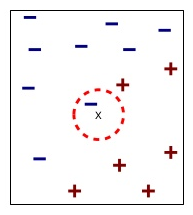
\includegraphics[width=\textwidth]{knna}
        \caption{\textit{k}=1}
        \label{fig:knna}
    \end{subfigure}
    \hfill
    \begin{subfigure}[b]{0.3\textwidth}
        \centering
        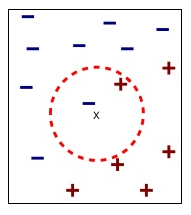
\includegraphics[width=\textwidth]{knnb}
        \caption{\textit{k}=2}
        \label{fig:knnb}
    \end{subfigure}
    \hfill
    \begin{subfigure}[b]{0.3\textwidth}
        \centering
        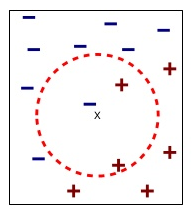
\includegraphics[width=\textwidth]{knnc}
        \caption{\textit{k}=3}
        \label{fig:knnc}
    \end{subfigure}
    \caption{Susedstva i dodeljivanje klasa novoj instanci za \textit{k}=1, 2 i 3}
    \label{fig:knn}
\end{figure}

Na slici \ref{fig:knn} prikazana su susedstva instance koja se nalazi u sredini kruga kada algoritam \textit{k} najbližih suseda uzima vrednosti 1, 2 i 3 za \textit{k}. Instanci će biti dodeljena klasa na osnovu klasa njenih najbližih suseda. Na slici \ref{fig:knna} klasa najbližeg suseda je (-) pa će i klasa instance biti (-). U slučaju \ref{fig:knnc} dva suseda su klase (+), a jedan klase (-) pa će klasa instance biti (+). Slika \ref{fig:knnb} ilustruje situaciju podjednake zastupljenosti klasa (jedan (+) i jedan (-)). U ovakvim situacijama, instanci se dodeljuje klasa slučajnim izborom \cite{mitic}.

Za rezultat klasifikacije jako je bitan izbor parametra \textit{k}. U slučaju male vrednosti parametra \textit{k} može doći do preprilagođavanja. Do grešaka dolazi jer je mali broj suseda uključen u razmatranje. Često se može javiti greška zbog prisustva šuma. Sa druge strane, velika vrednost parametra \textit{k} vodi ka \textit{potprilagođavanju} (eng.~model underfitting) - situaciji kada model loše klasifikuje i trening i test podatke zato što nije uspeo da nauči pravu strukturu podataka sa kojima radi. U tom slučaju do greške može doći jer se razmatraju klase onih objekata koji nisu u neposrednom susedstvu. Izbor vrednosti parametra $k$ je, u praksi, vođen nekom heuristikom. Čest način izbora parametra je poređenjem tačnosti modela konstruisanih za različite vrednosti parametra $k$ \cite{mladen, mitic, aggarwal}.

%% LR
\subsection{Logistička regresija}

% probabilisticki modeli
Logistička regresija predstavlja probabilistički model klasifikacije. Koristi se i za probleme binarne i za probleme višeklasne klasifikacije. Kod probabilističkih modela je potrebno definisati raspodelu verovatnoće koju kasnije treba oceniti na osnovu podataka. Da bi ocena raspodele bila računski izvodljiva potrebno je uvesti pretpostavke o: (1) raspodeli podataka i (2) međusobnoj zavisnosti promenljivih. Pogrešne pretpostavke o podacima, njihovoj raspodeli i zavisnosti, vode ka lošijim rezultatima predviđanja. U daljem tekstu detaljnije je opisana binarna logistička regresija \cite{mladen}.

Logistička regresija pretpostavlja međusobnu nezavisnost vrednosti ciljne promenljive \textit{y} za date vrednosti atributa \textit{x} i \textit{Bernulijevu raspodelu} ciljne promenljive \textit{y} za date vrednosti atributa \textit{x}. To znači da postoji parametar  $\mu$ iz intervala [0,1] takav da je  \textit{p}(\textit{y}=1|\textit{x}) = $\mu$, a  \textit{p}(\textit{y}=0|\textit{x}) = 1-$\mu$. Ovako definisan model logističke regresije nije kompletan. Potrebno je definisati zavisnost parametra $\mu$ od vrednosti atributa \textit{x}. Da bi se parametar $\mu$ uklopio u definiciju verovatnoće, njegove vrednosti moraju biti u intervalu [0,1]. Poželjno bi bilo koristiti model linearne regresije zbog njegove jednostavnosti i lake interpretabilnosti. Međutim, na prvi pogled korišćenje linearnog modela nije moguće jer vrednosti linearnog modela pripadaju intervalu [$-\infty$, $\infty$]. Korišćenje modela linearne regresije je moguće ako se njegove vrednosti transformišu nekom nenegativnom, monotonom, neprekidnom i diferencijabilnom funkcijom u interval [0,1]. U tu svrhu koristi se \textit{sigmoidna funkcija} $\sigma$ (moguća je upotreba i nekih drugih funkcija):
$$ \sigma(t) = \frac{\mathrm{1}}{\mathrm{1} + e^{(- t)}} $$
Sigmoidna (logistička) funkcija, čiji je grafik prikazan na slici \ref{fig:sigmagraph}, uzima proizvoljan realan broj i dodeljuje mu vrednost iz intervala (0,1). 

\begin{figure}[!ht]
  \centering
  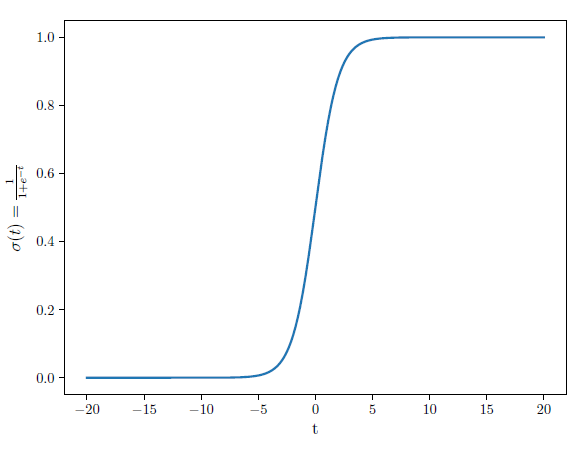
\includegraphics[width=0.8\textwidth]{sigma.png}
  \caption{Sigmoidna funkcija}
  \label{fig:sigmagraph}
\end{figure}

Transformacijom vrednosti linearnog modela, definisana je i zavisnost parametra Bernulijeve raspodele $\mu$ od vrednosti atributa \textit{x}. Slično modelu linearne regresije, forma modela logističke regresije je jednačina: $$  p_w (y=1|x) = \sigma(w \cdot x) $$Izlaz modela je linearna kombinacija njegovog ulaza i koeficijenata. Koeficijenti se dobijaju iz podataka prilikom samog treniranja modela i oni predstavljaju reprezentaciju modela u memoriji \cite{mladen, mlm}.

Treniranje modela linearne regresije odgovara oceni njegovih parametara i zasniva se na \textbf{principu maksimalne verodostojnosti}. Kao što smo videli, da bi se precizirao statistički model potrebno je uključiti neke parametre. Da bi dobijeni rezultat imao smisla, izbor vrednosti parametara je jako bitan. Jedan od principa izbora ovih vrednosti, princip maksimalne verodostojnosti, je prihvatanje onih vrednosti parametara za koje su posmatrani podaci visoko verovatni \cite{mladen}.
%je neprihvatanje onih vrednosti parametara za koje su posmatrani podaci malo verovatni. Na taj način biće prihvaćene one vrednosti parametara za koje su posmatrani podaci visoko verovatni \cite{mladen}.

%% RF
\subsection{Slučajne šume}

\textit{Ansambl metodi (eng.~ensemble methods)} su tehnike koje za cilj imaju poboljšanje tačnosti klasifikacije koje se postiže kombinovanjem predviđanja većeg broja klasifikatora. Ovi metodi konstruišu veći broj \textit{baznih klasifikatora} (eng.\textit{ base classifiers}) i kombinovanjem njihovih rezultata vrše svoje predviđanje. Rezultat predviđanja je srednja vrednost u slučaju regresije ili najzastupljenija vrednost u slučaju klasifikacije. Rezultati dobijeni primenom ansambl klasifikatora mogu biti bolji od rezultata dobijenih korišćenjem samo jednog klasifikatora ako su ispunjena sledeća dva uslova \cite{mitic}:
\begin{enumerate}[1)]
\item Bazni klasifikatori treba da budu međusobno nezavisni. 
U tom slučaju bi, za problem binarne klasifikacije, konačna predikcija bila pogrešna samo ako više od polovine baznih klasifikatora pogreši u predikciji. Potpuna nezavisnost klasifikatora je teško ostvariva, ali se u praksi pokazalo da nije neophodna da bi se ostvarili bolji rezultati. 
\item Bazni klasifikatori treba da budu bolji od slučajnog klasifikatora.
\end{enumerate}

Osnovna ideja ansambl metoda je kreiranje velikog broja klasifikatora na osnovu trening podataka i neki vid agregacije njihovih rezultata u slučaju nepoznate instance. Ansambl klasifikatora može se konstruisati na neki od sledećih načina \cite{mitic}:
\begin{description}
\item[Manipulacijom trening podataka] Ponovnim izborom, u skladu sa izabranom raspodelom, iz originalnog skupa trening podataka kreira se veći broj novih skupova podataka. Raspodela utiče na verovatnoću da će podatak biti izabran za novi trening skup. Zatim se za svaki novi trening skup kreira model klasifikacije izabranim algoritmom (npr. stablo odlučivanja). Dva ansambl metoda koja rade na ovaj način su upakivanje i podsticanje.
\begin{description}
\item[Upakivanje] (eng.~\textit{bagging}) je tehnika koja iznova vrši izbor uzoraka sa zamenom na osnovu uniformne raspodele verovatnoća. Kako sve instance imaju jednaku verovatnoću da budu izabrane, ova tehnika je manje podložna greškama usled preprilagođavanja. Dobijeni skup uzoraka je iste veličine kao i originalni skup. Kako se izbor uzoraka vrši sa zamenom neki podaci će biti izabrani više puta a neki nijednom. Na dobijenim skupovima se treniraju klasifikatori. Nakon što se kreiraju svi klasifikatori moguće je klasifikovati nepoznate instance. Dodeljivanje klase nepoznatoj instanci vrši se tako što svaki bazni klasifikator d\^a svoju predikciju klase, nakon čega se novoj instanci pridružuje najzastupljenija klasa.
\item[Podsticanje] (eng.~\textit{boosting}) je iterativna procedura koja postepeno menja raspodelu trening podataka i na taj način favorizuje one podatke koji su teži za klasifikaciju. Svakoj trening instanci je pridružen koeficijent težine koji se može promeniti po završetku iteracije. Težine se mogu koristiti bilo kao raspodela pri kreiranju novih skupova podataka bilo za treniranje pristrasnih modela.
\end{description}
\item[Manipulacijom ulaznih atributa] Novi skupovi trening podataka nastaju kao podskupovi originalnih podataka, slučajnim izborom podataka početnog skupa ili analizom domena. Ovaj pristup daje dobre rezultate u slučaju redundantnih atributa. Slučajne šume su primer metoda koji manipuliše ulaznim atributima i koristi klasifikatore zasnovane na stablima odlučivanja u svojoj osnovi. 
\item[Manipulacijom algoritma učenja] Moguće je menjati i sam algoritam učenja. Ovaj način nalazi praktičnu primenu ubacivanjem faktora slučajnosti prilikom treniranja skupa stabala odlučivanja. Umesto izbora najboljeg atributa za podelu u čvoru, moguće je slučajnim izborom odabrati jedan od nekoliko najboljih atributa podele.
\item[Manipulacijom oznaka klasa] Ako je broj klasa dovoljno veliki, višeklasni problem je moguće transformisati u binarni problem podelom oznaka klasa, na slučajan način, u dva disjunktna skupa $A_0$ i $A_1$. Trening podacima čije klase pripadaju skupu $A_0$ pridružuje se klasa 0, a podacima čije klase pripadaju skupu $A_1$ klasa 1. Podaci sa novim oznakama klasa se koriste za treniranje baznog klasifikatora. Ansambl klasifikatora se dobija višestrukim ponavljanjem kreiranja skupova $A_0$ i $A_1$ i treniranja klasifikatora nad dobijenim skupovima. Dodeljivanje klase nepoznatoj instanci vrši se tako što svaki bazni klasifikator $C_i$ vrši predviđanje. Ako je predviđena klasa 0, sve klase skupa $A_0$ dobijaju glas. Analogno, ako je predviđena klasa 1, sve klase skupa $A_1$ dobijaju glas. Glasovi se prebrojavaju i rezultujuća klasa će biti ona sa najviše glasova. \par
\end{description}


% naci ovo u miticevoj knjizi
%Slučajne šume nalaze praktičnu primenu zbog otpornosti na greške usled preprilagođavanja koje su karakteristične za stabla odlučivanja. \textit{Stabla odlučivanja (eng. Decision trees)} su popularan metod za rešavanje brojnih problema mašinskog učenja. Često se koriste zbog svoje skalabilnosti, interpretabilnosti i robusnosti pri korišćenju nebitnih atributa. Međutim, stabla odlučivanja su retko tačna. Stabla razvijena previše u dubinu često imaju grešku nastalu preprilagođavanjem. Iako nisu pristrasna, imaju visoku varijansu. Slučajne šume nastaju sa ciljem smanjenja varijanse. Posledica ovoga su nešto veća pristrasnost modela i gubitak interpretabilnosti, ali i znatno poboljšanje performansi izračunavanja. [mitic, wiki-random-forrest]

%Stabla odlučivanja su jednostavna tehnika mašinskog učenja koja ima široku primenu zbog brojnih prednosti. Ovi modeli su jednostavni i jeftini za implementaciju, lako se interpretiraju, robusni su na uticaj šuma, prisustvo redundantnih podataka ne utiče na tačnost modela. Sa druge strane, stabla razvijena previše u dubinu često imaju grešku nastalu preprilagođavanjem

\textit{Slučajne šume} (eng.~\textit{Random forests}) pripadaju klasi ansambl metoda. Kao bazni klasifikatori se koriste stabla odlučivanja koja se konstruišu nad skupom nezavisnih slučajnih vektora koji nastaju metodom manipulacije trening podataka. \textit{Upakivanje sa korišćenjem stabala odlučivanja} (eng.~\textit{Bagging using decision trees}) je specijalan slučaj slučajnih šuma u kom se slučajnost dodaje u proces pravljenja modela (do sada je postojala u trening podacima) tako što se novi skupovi podataka kreiraju metodom slučajnog izbora sa zamenom od elemenata polaznog skupa. Dodavanje slučajnosti smanjuje korelaciju između stabala, a samim tim i grešku generalizacije ansambla. %cele grupe. 
Upakivanje popravlja grešku generalizacije smanjujuću varijansu baznih klasifikatora. Pored toga, upakivanje je manje podložno i greškama usled preprilagođavanja, koje je velika mana stabala odlučivanja, zato što nijedna trening instanca nema prednost prilikom izbora, već sve imaju podjednaku verovatnoću da će biti izabrane \cite{mitic}.

%Greška pri generalizaciji teži da raste sa porastom korelacije između stabala. Korelacija među stablima nastaje kada je jedan atribut jak prediktor izlaza. U tom slučaju atribut će se naći u velikom broju stabala, a posledica toga je korelacija među njima.
Svako stablo odlučivanja za podelu u čvoru koristi odgovarajući slučajni vektor podataka koji se dobija na jedan od sledećih načina \cite{mitic}:
\begin{enumerate}[1)]
\item Slučajnim izborom se određuje $F$ atributa koji će se koristiti za podelu u svakom od čvorova (umesto da se za podelu razmatraju svi atributi) nakon čega se stablo konstruiše do kraja bez odsecanja. Ako postoji potreba za većim faktorom slučajnosti moguće je koristiti upakivanje za kreiranje trening skupova. Izbor broja atributa $F$ utiče na snagu i korelaciju modela slučajnih šuma. Za male vrednosti $F$ stabla šume su slabo korelisana, dok veliko $F$ omogućava jače modele zbog korišćenja većeg broja atributa. Često se kao kompromisno rešenje za broj atributa uzima $F=log_2d+1$, gde je $d$ broj ulaznih atributa. Ovaj pristup vodi manjem vremenu izvršavanja algoritma jer se prililkom podele u čvoru ne razmatraju svi atributi. 
\item Ako početnih atributa $d$ ima malo, teško je pronaći nezavisni skup slučajnih atributa koji se koriste pri izgradnji modela. Ovo se može prevazići proširenjem skupa atributa njihovom linearnom kombinacijom. Na nivou svakog čvora novi atribut nastaje tako što se metodom slučajnog izbora izabere $L$ atributa iz polaznog skupa, nakon čega se ti atributi linearno kombinuju sa koeficijentima dobijenim iz uniformne raspodele na intervalu [-1,1]. Svaki čvor će dobiti $F$ novih atributa, a najbolji od njih će biti korišćen za podelu čvora. 
\item Mogući pristup podeli unutar čvora je da se umesto najboljeg atributa podele na slučajan način izabere jedan od $F$ najboljih atributa. Stabla dobijena na ovaj način mogu imati veći stepen korelacije u slučaju nedovoljno velikog parametra $F$. Pored toga, ovaj pristup ne daje uštedu u vremenu izvršavanja kao prethodna dva pristupa jer je potrebno ispitati svaki atribut podele u svakom čvoru stabla. 
\end{enumerate}

\section{Mašinsko učenje u Python-u}
,,Python je interpretirani, objektno-orijentisani viši programski jezik sa dinamičkom semantikom. Pythonova jednostavna sintaksa se lako uči i naglašava čitljivost koda koja za posledicu ima nisku cenu održavanja \cite{python-blurb}''. Python podržava veliki broj paketa i modula što vodi ponovnoj upotrebljivosti i modularnosti koda. Nepostojanje faze kompilacije ubrzava čitav proces pisanja i testiranja koda. Debagovanje je prilično jednostavno, greške proizvode izuzetke i ako se oni ne uhvate interpreter ispisuje \textit{stanje steka} (eng.~\textit{stack trace}). Štaviše, često je najjednostavniji način debagovanja ubacivanje print naredbi \cite{python-blurb}. %https://www.python.org/doc/essays/blurb/

Autor Pythona je Holanđanin Gido Van Rosum (hol. Guido Van Rossum). Ideju o Pythonu dobija krajem 1980-ih kada je radio kao programer na Državnom institutu za matematiku i informatiku CWI (Centrum voor Wiskunde en Informatica) u jeziku ABC kojim je inspirisan. Implementaciju započinje decembra 1989-te, a prva verzija jezika (verzija 0.9.0) puštena je 1991-ve. Januara 1994-te izlazi verzija 1.0 koja se razvija sve do septembra 2000-te. Unapređena verzija 2.0 (poznata i kao Python 2) izlazi u oktobru 2000-te, a verzija 3.0 (Python 3) u decembru 2008-me. Zanimljivo je da razvoj verzije 2.0 nije zaustavljen izlaskom nove velike verzije 3.0. Razlog za to je činjenica da je Python 3 prva distribucija namerno napravljena da bude nekompatibilna sa prethodnim distribucijama. Poslednja i konačna verzija vezana za Python 2 je 2.7 iz jula 2010-te, koja je i dalje podržana (poslednja promena desila se u aprilu 2018-te (2.7.15)). Verzija 3.7.0 je najnovijeg datuma (jun 2018-te). Izmene koje Python 3 donosi su brojne, a neke od njih su: print više nije naredba već postaje funkcija, interfejsi poput rečnika i mapa vraćaju poglede i iteratore umesto listi, pojednostavljena su pravila operatora poređenja, napravljene su promene u samoj sintaksi,...  \cite{python-history, python-dates, python-whats-new}.
% https://legacy.python.org/doc/essays/foreword/  
% https://www.python.org/doc/versions/   		

\subsection{SciPy ekosistem}
 
\textbf{SciPy} je ekosistem slobodnog softvera za matematiku, nauku i inženjerstvo. Njegovu osnovu čini programski jezik Python i grupa paketa od kojih su za mašinsko učenje najznačajniji \cite{scipy}:
\begin{enumerate}[1)]
\item \textbf{NumPy} je osnovni paket za naučna izračunavanja u Pythonu. Ovaj paket definiše numeričke nizove, matrične tipove, kao i osnovne operacije nad njima.  %https://www.scipy.org/about.html]
%https://docs.scipy.org/doc/numpy/user/quickstart.html
Glavni objekat paketa je homogeni višedimenzioni niz koji je predstavljen kao tabela elemenata (najčešće brojeva), pri čemu su svi istog tipa i indeksirani torkom pozitivnih celih brojeva. Dimenzije niza se nazivaju \textit{osama} (eng.~\textit{axis}). Klasa nizova NumPy paketa se naziva \textit{ndarray}.
\begin{itemize}
\item Tačka prostora npr. [1, 2, 1] sa svoje tri koordinate ima jednu osu (dimenziju). Osa se sastoji od 3 elementa pa se kaže da je dužine 3. 
\item Dvodimenzioni niz, npr.
$$[[ 1., 0., 0.],$$ 
$$ [ 0., 1., 2.]] $$
 ima dve ose. Prva osa ima 2 elementa, a druga 3 \cite{scipy, scipy-quickstart}. 
\end{itemize}
\item \textbf{Pandas}  %https://pandas.pydata.org/pandas-docs/stable/
je paket koji obezbeđuje strukture podataka za jednostavan i intuitivan rad sa podacima. Predstavlja nadgradnju NumPy biblioteke i napravljen je tako da se lako integriše u razna okruženja koja se koriste za naučna izračunavanja. Pogodan je za podatke koji su smešteni u tabelama, uređene i neuređene vremenske serije, proizvoljne matrice i sve oblike podataka dobijenih na osnovu statističkih posmatranja. Pandas uvodi dve strukture podataka, Series za jednodimenzione podatke i DataFrame za dvodimenzione \cite{pandas}. 
\item \textbf{Matplotlib}  %https://matplotlib.org/ 
je biblioteka koja služi za kreiranje različitih vrsta dijagrama. Većinu dijagrama moguće je kreirati u svega nekoliko linija koda, a sami dijagrami se mogu prilagoditi potrebama korisnika izborom stilova linija (pune, isprekidane,...), svojstava fontova, svojstava koordinatnih osa, itd \cite{matplotlib}.
\end{enumerate}

\textbf{Scikit-learn}  %http://scikit-learn.org/stable/index.html
je modul koji implementira veliki broj algoritama mašinskog učenja. Pored algoritama za rešavanje problema klasifikacije, regresije i klasterovanja ovaj modul podržava i razne tehnike preprocesiranja podataka, kao i tehnike ocenjivanja modela. Zasniva se na bibliotekama NumPy, SciPy i matplotlib \cite{scikit-learn}.



\chapter{Verifikacija softvera}

Softver se nalazi svuda oko nas. U svakodnevnom životu, ljudi se sve više oslanjaju na sisteme zasnovane na informacionim i komunikacionim tehnologijama, pri čemu ti sistemi postaju sve složeniji i sve zastupljeniji. Ovi sistemi nalaze primenu u velikom broju oblasti: od berze, preko telefonskih i internet tehnologija pa sve do medicinskih sistema. Osim što se od njih očekuju dobre performanse u smislu vremena odziva i izračunavanja, jedan od ključnih aspekata kvaliteta sistema je odsustvo grešaka. Međutim, softver je pisan od strane ljudi pa stoga ne može biti savršen i podložan je greškama \cite{PoMC, SoftTest}.

Neke greške mogu biti pogubne po proizvođače. Greška pri deljenju brojeva u pokretnom zarezu na Intelovom Pentium II čipu (Intel Pentium Floating-Point Division Bug) ranih 1990-ih izazvala je gubitak od oko 475 miliona dolara da bi se čip zamenio i narušila je reputaciju Intela kao proizvođača pouzdanih čipova. Softverska greška u sistemu za upravljanje prtljagom prouzrokovala je odlaganje otvaranja aerodroma u Denveru za 9 meseci, što je dovelo do gubitka od 1,1 milion dolara po danu. Prestanak rada sistema za rezervaciju karata svake aviokompanije na svega 24 časa bi doveo kompaniju do bankrota zbog propuštenih porudžbina. NASA-ina kosmička letelica (NASA Mars Polar Lander) je usled nedovoljno testiranja 1999-te prilikom pokušaja sletanja prevelikom brzinom udarila u površinu Marsa i raspala se. Nekoliko stotina milijardi dolara potrošeno je za ispravljanje baga Y2K (The Y2K (Year 2000) Bug \cite{y2k}) \cite{PoMC, SoftTest}. 

Neke druge greške imaju daleko ozbiljnije posledice i njihova cena se ogleda u ljudskim životima. Softveri se koriste za upravljanje sistemima kao što su hemijske i nuklearne elektrane, sistemima za upravljanje saobraćaja, sistemima za odbranu od olujnih talasa (eng.~storm surge barriers), a greške ovih sistema mogu imati katastrofalne posledice. Greška u protivraketnom sistemu (Patriot Missile Defense System) 1991-ve dovela je do smrti 28 vojnika. Greška u mašini za terapiju radijacijom Therac-25 prouzrokovala je smrt šest pacijenata u periodu između 1985-te i 1987-me zbog prevelike izloženosti radijaciji  \cite{PoMC, SoftTest}.

\section{Specifikacija}

Provera ispravnosti nekog softvera, odnosno njegovog ponašanja, nije moguća bez poznavanja željenog ponašanja datog softvera. Sa ciljem definisanja željenog ponašanja uvodi se pojam specifikacije. \textit{Specifikacija} predstavlja dogovor razvojnog tima oko toga šta softver treba da radi. 

Rezultat ispitivanja zahteva klijenta su podaci koji opisuju šta klijent očekuje od programa. Ovi podaci ne opisuju proizvod koji treba napraviti. Opis proizvoda se zadaje specifikacijom. Za formulisanje specifikacije koriste se informacije dobijene od klijenta ali specifikacija obuhvata i zahteve koje program mora da ispuni a koje klijent nije naveo. Preciznost specifikacije može da varira. Kompanije koje razvijaju proizvode u oblastima medicine, vazduhoplovstva, kao i za vladine organizacije koriste striktniji oblik specifikacije koji podrazumeva veliki broj provera. Rezultat je iscrpna i temeljna specifikacija koja se ne može menjati, osim pod ekstremnim okolnostima i svaki član razvojnog tima tačno zna šta treba da napravi. Sa druge strane, kompanije koje razvijaju programe čija je primena u manje rizičnim oblastima primenjuju neformalniji vid specifikacije ili je uopšte ne primenjuju. Prednost ovakvog pristupa pisanju specifikacije ogleda se u fleksibilnosti, ali je veliki nedostatak potencijalna neusklađenost oko ponašanja programa kao i to što se sve do završetka projekta ne zna kako će njegova finalna verzija izgledati \cite{mvj, SoftTest}.

% ,,Specifikacija daje opis šta softver treba da radi \cite{mvj}''. 

\section{Verifikacija i validacija}

Verifikacija i validacija su pojmovi koji se često međusobno prepliću a imaju različito značenje. \textit{Verifikacija} (eng.~software verification) je postupak potvrđivanja da softver zadovoljava specifikaciju. \textit{Validacija} (eng.~software validation) je postupak potvrđivanja da softver zadovoljava potrebe korisnika. % mozda ne treba da bude pod navodnicima
Razlika između ova dva slična pojma se može razjasniti na primeru problema sa Habl teleskopom (eng.~Hubble telescope). Habl je reflektujući teleskop koji koristi veliko ogledalo da uveća objekte ka kojima je uperen. Pravljenje ogledala je zahtevalo veliku tačnost i preciznost. Kako je ogledalo pravljeno da se koristi u svemiru, jedini način da se testira je bio pažljivim merenjem svih atributa ogledala i njihovim poređenjem sa specifikacijom. Testovi su prošli uspešno i teleskop je lansiran u zemljinu orbitu aprila 1990-te. Ubrzo nakon što je teleskop počeo sa radom otkriveno je da su slike koje vraća mutne kao posledica greške u specifikaciji. Iako je ogledalo zadovoljavalo specifikaciju, specifikacija je bila pogrešna što je dovelo do ogledala koje ima visoku preciznost a nisku tačnost. Testiranje je u ovom slučaju potvrdilo da ogledalo zadovoljava specifikaciju tj. verifikacija je bila uspešna. Sa druge stranje testiranje nije potvrdilo da ogledalo zadovoljava zahteve korisnika i validacija, da je rađena, ne bi prošla. Cena ove greške je bila u novoj svemirskoj misiji 1993-će da bi se dodalo korektivno sočivo \cite{SoftTest}.

Uopšteno govoreći, program ne zadovoljava specifikaciju ako sadrži greške koje narušavaju funkcionalne i nefunkcionalne željene osobine programa. Funkcionalne osobine definišu koji su to željeni izlazi za zadate ulaze, a u nefunkcionalne osobine softvera spadaju vreme odziva, performanse i efikasnost. Bitna klasa grešaka koje mogu da naruše funkcionalne osobine softvera je klasa grešaka koje utiču na ispunjavanje bezbednosnih zahteva, npr. dovode do kraha programa ili utiču na performanse i efikasnost. Neki od primera su pokušaj deljenja nulom, pokušaj dereferenciranja NULL pokazivača, pokušaj čitanja sadržaja van granica rezervisane memorije i prisustvo kružnih blokada. Ove greške se mogu javiti nevezano od namene programa  \cite{mvj}.

Osnovne vrste verifikacije softvera su dinamička i statička  \cite{mvj}. Ova dva pojma se slikovito mogu opisati na primeru kupovine polovnog automobila. Gledanje ispod haube, traženje tragova rđe, traženje ulubljenja, traženje ogrebotina na farbi, naprsnuća stakla, šutiranje guma su tehnike statičkog testiranja. Paljenje motora automobila i vožnja koja obuhvata dodavanje gasa i kočenje su tehnike dinamičkog testiranja \cite{SoftTest}.


\section{Dinamička verifikacija softvera}
Dinamička verifikacija softvera je provera njegove ispravnosti u toku izvršavanja. Provera ispravnosti se najčešće vrši testiranjem. Samim testiranjem se ne može dokazati ispravnost programa. Ono što testiranje može da uradi je da pokaže prisustvo grešaka, ne i njihovo odsustvo. Zbog toga je svrha testiranja otkrivanje grešaka koje program sadrži \cite{mvj}.  

Testiranje je proces u kojem se program pokreće sa reprezentativnim skupom ulaznih podataka, nakon čega se rezultati porede sa očekivanim. Strategija testiranja služi za određivanje reprezentativnih ulaza pri čemu reprezentativni skup treba da zadovoljava sledeće uslove: (1) ima visok potencijal otkrivanja greške, (2) relativno je male veličine, (3) vodi do visokog poverenja u softver nakog što softver uspešno prođe sve test primere. Dva osnovna izvora testova su programski k\^od i specifikacija programa. U zavisnosti od izvora testova postoje tri strategije testiranja \cite{mvj}:
\begin{description}
\item [Strategije testiranja crne kutije] (eng.~black-box testing) su strategije generisanja testova na osnovu specifikacije programa. Poznate su pod nazivima testiranje vođeno podacima ili testiranje vođeno ulazom i izlazom. Ideja je da se program posmatra kao crna kutija, sve se zasniva na zahtevima i specifikaciji programa, bez ikakvih briga o njegovoj strukturi i unutrašnjem ponašanju. Fokus strategije je na pronalaženju uslova koji dovode do ponašanja programa koje je suprotno ponašanju navedenom u specifikaciji. Test primeri se izvode samo na osnovu specifikacije softvera. U okviru ovih strategija izdvajaju se testiranje funkcionalnih i nefunkcionalnih osobina softvera, kao i regresiono testiranje \cite{mvj, ArtOfST, PGtSTD}.

Da bi se ovom strategijom pronašle sve greške koje postoje u programu potrebno je testirati svaki mogući ulaz u program. \\
Za testiranje programa koji rešava problem trouglova (za date celobrojne vrednosti stranica trougla program daje odgovor na pitanje da li je trougao jednakokraki, jednakostranični ili nejednakostranični \cite{schlingloff} %[Prof. Dr. Holger Schlingloff]
) potrebno je testirati sve validne i nevalidne trouglove. Skup celobrojnih vrednosti je sam po sebi ogroman, uz nevalidne ulaze broj ulaza koje treba proveriti se drastično povećava.\\
Iscrpno testiranje velikih programa predstavlja jos veći problem. Da bi se testirala ispravnost kompajlera potrebno je kao ulaz koristiti ne samo svaki validni program (kojih ima beskonačno), već i svaki nevalidni program (kojih takođe ima beskonačno). Tek tada bi se sa sigurnošću moglo tvrditi da kompajler neće uspešno prevesti neispravan program. A ovo je samo jedna osobina kompajlera. Postoji veliki broj relevantnih osobina kompajlera koje bi takođe trebalo utvrditi na isti način (npr. da je zadržana semantika izvornog programa - ako u programu imamo $a+b$ da je to prevedeno u $add$ $a, b$ a ne u $sub$ $a, b$)). \\
Stvari se dodatno komplikuju kod programa koji koriste neki oblik memorije poput aplikacija koje rade sa bazama podataka. U slučaju sistema za rezervaciju avionskih karata izvršavanje jedne transakcije (na primer, provera slobodnih mesta čitanjem iz baze, rezervacija karte upisom u bazu) zavisi od toga šta se desilo u prethodnim transakcijama. Stoga je potrebno proveriti ne samo sve moguće validne i nevalidne transakcije već i sve moguće sekvence transakcija \cite{ArtOfST}.

Prethodni primeri pokazuju da je iscrpno testiranje nemoguće zbog beskonačnog skupa test primera. Pošto je prostor mogućih ulaza u program veliki, bira se njegov podskup. Veliki nedostatak ove strategije je i što osoba koja testira softver ne može da zna koliki je procenat softvera testiran. Takođe, postoji opasnost da neke putanje izvršavanja nikad ne podlegnu testiranju. Sa druge strane, ovakav pristup testiranja pomaže testeru da izabere konačne podskupove ulaza (test primera) na osnovu kojih će se pronaći što veći broj grešaka \cite{ArtOfST, PGtSTD}.

\item [Strategije testiranja bele kutije] (eng.~white-box testing) su strategije kod kojih se testiranje zasniva na poznavanju unutrašnjih putanja, strukture i implementacije koda. Informacije dobijene na osnovu gledanja koda programa koriste se da bi se donela odluka o tome šta testirati i kako pristupiti testiranju i sami testovi se generišu na osnovu programskog koda. Nazivaju se i strategijama strukturnog testiranja (eng.~structural testing) zato što se testovi kreiraju i izvršavaju na osnovu posmatranja strukture koda. Najčešći primer ovakvog testiranja su jedinični testovi (testovi jedinica koda). Ideja ove strategije je da se napravi paralela sa strategijom crne kutije pri čemu se test primeri dobijaju iz strukture softvera. Osnovne strategije strukturnog testiranja zasnivaju se na kriterijumu pokrivenosti koda (eng.~code coverage). Pokrivenost se može računati prema broju izvršenih putanja kroz program, broju instrukcija, broju grana nakon svake instrukcije grananja ili kombinacijom prethodnih kriterijuma. Smatra se da je pomenuta paralela sa strategijom crne kutije iscrpno testiranje putanja kroz program) \cite{PGtSTD, SoftTest, mvj, ArtOfST}. 

Slično strategijama crne kutije i ovde postoje nedostaci: (1) broj jedinstvenih logičkih putanja kroz program može biti ogroman i (2) čak iako se testiraju sve putanje moguće je da program sadrži greške. Ovo se može desiti iz jednog od tri razloga: (1) iscrpno testiranje putanja ne daje garanciju da program zadovoljava specifikaciju (pri pisanju programa koji uređuje neke vrednosti u rastućem poretku moguće je napraviti grešku i uređenje vršiti u opadajućem poretku), (2) moguće je da program ne radi kako treba zato što mu nedostaje neka putanja (neke nedostajuće putanje testiranje može da detektuje, a neke ne može) i (3) greške osetljive na podatke (eng.~data sensitive errors) mogu ostati neotkrivene (na primer, kod poređenja da li je razlika dva broja manja od neke vrednosti, računanje $a-b<c$ će sadržati greške zato što zapravo treba posmatrati apsolutnu vrednost razlike). Još jedan nedostatak je što osoba koja testira program, da bi isti razumela, mora da poseduje znanje iz oblasti programiranja. Prednost ove strategije je što se identifikuju i testiraju sve putanje kroz softver \cite{mvj, ArtOfST, PGtSTD}.

\item [Strategije testiranja sive kutije] (eng.~gray-box testing) predstavljaju mešavinu prethodnih strategija. U ovim strategijama se na softver i dalje gleda kao na crnu kutiju s tim što se pored toga ,,zaviri'' u  k\^od programa tj. koriste se i specifikacija i programski k\^od \cite{mvj, SoftTest}.
\end{description}

%Od velikog značaja je automatizacija procesa generisanja test primera i provere rezultata testiranja jer ubrzava i olakšava proces testiranja. Rasplinuto testiranje (eng.~fuzz testing) je tehnika koju je moguće u potpunosti automatizovati.  


\section{Statička verifikacija softvera}
Statička verifikacija softvera je provera njegove ispravnosti na osnovu koda, bez njegovog izvršavanja. Analiza koda može biti od strane ljudi ili automatizovana. 
% ovde moze deo o pregledima sa slajdova 04 ili iz ron patton software testing

% sa slajdova sta je automatizovana analiza 04 - jedna recenica


Neodlučivost halting problema (problem ispitivanja ispravnosti programa) predstavlja ograničenje za automatizaciju provere ispravnosti programa. Posledica neodlučivosti je da se osobine polaznog sistema mogu verno opisati neodlučivim teorijama, ali proces dokazivanja nije moguće automatizovati baš zbog neodlučivosti teorija. Delimično rešenje ovog problema je u korišćenju interaktivnih dokazivača teorema (eng.~interactive theorem provers) kao što su Isabelle i Coq. Korišćenjem ovih sistema moguće je pouzdano interaktivno dokazati razne osobine ispravnosti programa. Proverom samog dokaza dodatno se obezbeđuje najviši stepen pouzdanosti i sigurnosti u dokaz ispravnosti. Problem sa ovim sistemima je što zahtevaju ljudski rad zbog čega se ne koriste za čitave programe, već za njihove delove ili kompleksne osobine \cite{mvj}. 
Potpuna automatizacija procesa verifikacije moguća je ako se polazni sistem opiše nekom odlučivom teorijom, ali često pod pretpostavkom neograničenih resursa. Neograničeno vreme, kao i bilo koji drugi neograničeni resurs u praksi nisu mogući. Svaki konačan opis u okviru odlučive teorije je, u opštem slučaju, samo aproksimacija ponašanja polaznog sistema. Posledice aproksimacija su neprecizna analiza jer opis polaznog sistema nije veran i analiza koju za neke programe nije moguće završiti zbog nedostatka resursa ili u konačnom vremenu. 
Kvalitet analize tj. dobijanje preciznijih rezultata u konačnom vremenu i sa konačnim resursima, može se poboljšati dodavanjem obeležja (eng.~annotations). Obeležjima se dodaju informacije koje je teško ili nemoguće automatski izvesti. Takođe se dodaju i informacije koje je moguće automatski izvesti ali se dodavanjem tih informacija štedi na vremenu potrebnom za analizu. Obeležjima se najčešće zadaju invarijante petlji, kao i preduslovi i postuslovi funkcija \cite{mvj}. 
Potpuno automatizovani pristupi verifikaciji programa su simboličko izvršavanje, apstraktna interpretacija i proveravanje modela. 

\subsection{Simboličko izvršavanje}
\textit{Simboličko izvršavanje} (eng.~symbolic execution) predstavlja analizu programa u kojoj se umesto konkretnih prate simboličke vrednosti promenljivih. Ovakvom analizom se kreiraju simbolički izrazi koji opisuju određene putanje kroz program što omogućava istovremenu proveru svih ulaza koji prate istu putanju. Simboličko izvršavanje istovremeno ispituje veliki broj putanja izvršavanja bez potrebe za konkretnim ulaznim parametrima. Umesto toga, vrši se apstrakcija ulaznih vrednosti simbolima nakon čega se koriste rešavači ograničenja (eng.~constraint solvers) da bi se proizvele konkretne vrednosti ulaza koje dovode do grešaka. Simboličko izvršavanje je nastalo sredinom 1970-ih sa ciljem otkrivanja da li se u okviru softvera mogu narušiti određena svojstva, npr. deljenje nulom, pokušaj dereferenciranja NULL pokazivača... Kada se testiranjem uz korišćenje konkretnih vrednosti ulaza prođe kroz jednu putanju programa, ona je izvršena samo za te konkretne vrednosti. Nasuprot tome, kada se simboličkim izvršavanjem prođe kroz jednu putanju programa, ona je izvršena za sve moguće vrednosti koje prolaze kroz tu putanju. Zbog toga je ključna ideja omogućiti programu da koristi simboličke vrednosti \cite{mvj, SurveySymExec}. 

Ako simboličko izvršavanje pokaže da neka putanja zadovoljava uslove ispravnosti programa tada svi ulazi koji prolaze putanju zadovoljavaju uslove programa čime se znatno dobija na efikasnosti provere u odnosu na tehnike dinamičke analize. Problem sa ovim pristupom je broj mogućih putanja koji je često prevelik da bi se u potpunosti pretražio. Zbog toga simboličko izvršavanje svoju primenu češće nalazi  u pronalaženju grešaka nego u verifikaciji programa. Veoma važan faktor koji utiče na brzinu otkrivanja greške u programu je redosled ispitivanja putanja. Ako se greška javlja u putanji koja se ispituje prva vreme otkrivanja greške je minimalno. U slučaju da se greška javlja u putanji koja se poslednja analizira vreme otkrivanja greške će biti veliko, a moguće je i da se greška uopšte ne pronađe. Ako postoji veliki broj putanja kroz program može doći do isteka vremena predviđenog za analizu pre nego što se greška otkrije \cite{mvj}.


\subsection{Apstraktna interpretacija}
,,\textit{Apstraktna interpretacija} (eng.~abstract interpretation) tehnika je aproksimacije formalne semantike programa, tj. matematičkog modela ponašanja programa \cite{mvj}''. ,,Apstraktna interpretacija obuhvata procenu ponašanja programa na nekom apstraktnom domenu, sa ciljem dobijanja približnog rešenja \cite{AutoTechnFormSofVer}''. Apstraktni domen je aproksimacija reprezentacije skupova konkretnih vrednosti, a za slikanje konkretnih vrednosti u vrednosti apstraktnog domena koristi se funkcija apstrakcije \cite{AutoTechnFormSofVer}. Semantika programa je opisana domenom $D_c$ i relacijama nad domenom pri čemu se relacije mogu menjati tokom izvršavanja naredbi programa. Provera da li neko svojstvo važi nad domenom $D_c$ može biti problem u slučaju velikih programa jer veliki programi znače velike domene i veliki broj mogućih putanja kroz program. Dodatan problem predstavlja neodlučivost koja se može javiti u raznim kontekstima. Kao potencijalno rešenje nameće se aproksimacija domena $D_c$ apstraktnim domenom $D_a$. Apstraktni domen ne može biti precizan kao konkretni domen, ali može dati informacije o nekim svojstvima domena. Sa druge strane, apstrakcijom domena se mogu izgubiti važne informacije. Primer jedne apstrakcije bila bi apstrakcija beskonačnog domena celih brojeva koji se menja skupom znakova brojeva {+, -, 0 }. Ovakva apstrakcija bi verno prikazala znak rezultata množenja dva cela broja ako su poznati samo znaci operanada. Ako je informacija od značaja znak rezultata sabiranja dva cela broja, pri čemu su poznati samo znaci operanada, ovakva apstrakcija se u nekim slučajevima pokazuje kao nedovoljna (znak rezultata sabiranja brojeva -3 i 5 je (+), a znak rezultata sabiranja brojeva -7 i 5 (-) ) \cite{mvj}. 


\subsection{Proveravanje modela}

\textit{Proveravanje modela} (eng.~model checking) je metod verifikacije u kojem se sistem, hardverski ili softverski, koji je potrebno verifikovati opisuje konačnim aparatom (stanjima i tranzicijama između stanja), a specifikacija se zadaje u terminima temporalne logike (specifikacija je opisana kao logička formula). U temporalnoj logici je moguće razmatrati uređenje događaja u toku vremena. Na primer, moguće je da trenutno netačno svojstvo postane tačno u nekom trenutku u budućnosti. Stanje modela čine vrednosti promenljivih i stanja steka i hipa, a tranzicije opisuju kako program prelazi iz jednog stanja u drugo stanje. Metodi zasnovani na proveravanju modela ispituju stanja programa do kojih se može doći. Nakon što je sistem opisan, stanja automata se obilaze sa ciljem dokazivanja uslova specifikacije. Proveravanje modela metodom grube sile istražuje sva moguća stanja sistema na sistematičan način, slično programu za igranje šaha. Na ovaj način je moguće dokazati da sistem zadovoljava neko svojstvo. Međutim, sa trenutno raspoloživim procesorima i memorijama ispitivanje najvećih mogućih prostora stanja predstavlja izazov. Najbolji programi za proveravanje modela mogu da rade sa prostorima stanja reda $10^8$ do $10^9$, a korišćenjem pametnih algoritama i specijalnih struktura za konkretne probleme prostor stanja može drastično da se uveća ($10^{20}$ do $10^{476}$!). Metod proverava da li sva relevantna stanja sistema zadovoljavaju željena svojstva. Ako je prostor stanja konačan metod će se izvršiti u konačnom vremenu. U slučaju neuspeha tj. ako se pronađe stanje koje narušava svojstvo koje se razmatra, generiše se kontraprimer koji definiše putanju izvršavanja koja vodi od inicijalnog stanja sistema do stanja kojim je svojstvo koje se proverava narušeno. Mana proveravanja modela je eksplozivan porast stanja tj. broj mogućih stanja eksponencijalno raste sa porastom broja promenljivih (komponenti sistema). Zbog toga se koristi metod proveravanja ograničenih modela \cite{mvj, AutoTechnFormSofVer, BMCUSS, PoMC}.

\textit{Proveravanje ograničenih modela} (eng.~bounded model checking)  je formalna tehnika verifikacije koja se mahom koristi u industriji poluprovodnika. Proveravanje ograničenih modela vrši brzu pretragu prostora stanja i za određene probleme daje znatno poboljšanje performansi izračunavanja u odnosu na metod proveravanja modela. Uspeh tehnike zasnovan je na velikim mogućnostima iskaznih SAT rešavača (eng.~propositional SAT solvers). Ovaj metod se zasniva na ograničavanju dužine putanje stanja koja se proverava. Ako se za zadatu vrednost dužine ne pronađe greška moguće je povećati vrednost tako da se provera nastavlja dok se ne pronađe greška, model ne postane prevelik za analizu ili vrednost dužine ne dostigne gornju granicu dužine mogućih putanja čime je model verifikovan  \cite{mvj, AutoTechnFormSofVer, BMCUSS}.

% \section{Neki verifikacijski alat}
% DODATI TEKST


%----------------------------

\chapter{Implementacija}
% DODATI UVODNI TEKST
%U ovom delu prikazani su postupak dobijanja najboljeg klasifikacionog modela i 

\section{Korišćeni podaci}
\label{kor_podaci}

Kao skup podataka za obučavanje modela klasifikacije korišćen je jm1.arff korpus podataka koji se nalazi na PROMISE repozitorijumu. PROMISE repozitorijum (eng.~PROMISE Software Engineering Repository) sadrži kolekciju javno dostupnih skupova podataka i alata koji treba da olakšaju istraživačima konstrukciju prediktivnih modela \cite{promise}. 

JM1 datoteka sadrži informacije o C programima, njihovim karakteristikama i o tome da li sadrže grešku ili ne. Sastoji se od 10878 objekata, od kojih svaki ima 22 atributa\footnote{Za potrebe ovog rada korišćeno je 18 atributa.  Izostavljeni su atributi cyclomatic complexity, design complexity, essential complexity i branch count. Ovi atributi su izostavljeni jer za njih nije pronađen jedinstven opis, a izborom atributa je utvrđeno da ne spadaju u 10 najbitnijih atributa pa bi pokušaj njihovog izračunavanja odneo previše vremena ili bio nemoguć a dobit bi bila sitna. Atributi su izostavljani tek nakon što je utvrđeno da njihovo izostavljanje neće značajno uticati na kvalitet modela klasifikacije - model dobijen bez ovih atributa ima preciznost svega 0,02 manju od modela koji koristi sve atribute. Zbog toga je procenjeno da je bolje poboljšavati model na druge načine. }. Sedamnaest atributa se odnosi na razne karakteristike koda, a osamnaesti je atribut klase ( da li program ima ili nema grešku) \cite{jm1}: 

\textbf{LOC\_BLANK numeric } Broj praznih linija u izvornom kodu programa

\textbf{LOC\_CODE\_AND\_COMMENT numeric} Broj linija koda i komentara

\textbf{LOC\_COMMENTS numeric} Broj linija komentara

\textbf{LOC\_EXECUTABLE numeric} Broj izvršivih linija koda

\textbf{LOC\_TOTAL numeric} Ukupan broj linija koda

\textbf{NUM\_OPERATORS numeric} $N_1$ Ukupan broj operatora u programu

\textbf{NUM\_OPERANDS numeric} $N_2$ Ukupan broj operanada u programu

\textbf{NUM\_UNIQUE\_OPERATORS numeric} $\eta_1$ Broj jedinstvenih operatora u programu

\textbf{NUM\_UNIQUE\_OPERANDS numeric} $\eta_2$ Broj jedinstvenih operanada u programu

\textbf{HALSTEAD\_CONTENT numeric} $I = L*V$

\textbf{HALSTEAD\_DIFFICULTY numeric} $D = 1/L = (\eta_1/2)*(N_2/\eta_2))$

\textbf{HALSTEAD\_EFFORT numeric} $E = V/L = D*V$

\textbf{HALSTEAD\_ERROR\_EST numeric} $B = V/3000$

\textbf{HALSTEAD\_LENGTH numeric} $N = N_1+N_2$

\textbf{HALSTEAD\_LEVEL numeric} $L = (2*\eta_2)/(\eta_1*N_2)$

\textbf{HALSTEAD\_PROG\_TIME numeric} $T = E/18$

\textbf{HALSTEAD\_VOLUME numeric} $V = (N_1+N_2)*(log_2(\eta_1+\eta_2))*N*log_2(n)$

\textbf{Defective \{Y,N\} } Atribut klase sa vrednostima $Y$ (program ima grešku) i $N$ (program nema grešku)

\subsection{Format arff}
% Data Mining Practical Machine Learning Tools and Techniques
ARFF (eng.~ Attribute-Relation File Format) predstavlja način reprezentacije skupova podataka koji se sastoje od nezavisnih, neuređenih instanci i koji ne uključuju međusobne relacije među instancama. Izgled arff fajla prikazan je na slici \ref{fig:arff}. Linije koje počinju znakom ,,\%'' predstavljaju komentare. Nakon komentara nalaze se naziv relacije i blok koji definiše atribute. Postoje četiri tipa atributa: imenski, brojčani, stringovi i datumi. Pri definiciji imenskih atributa potrebno je osim naziva atributa navesti i skup vrednosti, u vitičastim zagradama, koje atribut uzima. Brojčani atributi moraju da sadrže ključnu reč \textit{numeric}, stringovi \textit{string}, a datumi \textit{date}. Tip datum je zapravo poseban slučaj tipa string koji poštuje datum-vreme format: yyyy-MM-dd-THH:mm:ss (četiri cifre za godinu, po dve za mesec i dan nakon čega sledi ,,T'' i po dve cifre za sate, minute i sekunde). Odlika arff formata je da se klasni atribut eksplicitno ne navodi već je on jedan od navedenih atributa. Posledica ove odlike je da se isti fajl može koristiti da bi se odredilo koliko dobro se predviđa svaki atribut na osnovu ostalih, za pronalaženje pravila pridruživanja (eng.~association rules) ili za klasterovanje. Nakon bloka kojim se definišu atributi slede linije sa podacima, kojima prethodi @data linija. Svaka instanca se navodi u posebnoj liniji, vrednosti atributa su razdvojene zarezima, a nedostajuće vrednosti označene znakom ,,?'' \cite{weka}. 

\begin{figure}[!ht]
  \centering
  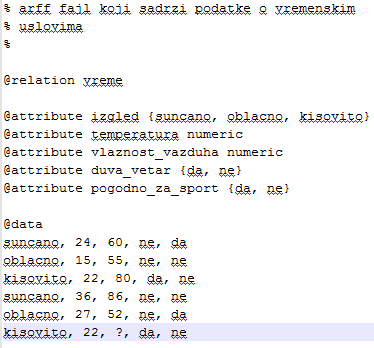
\includegraphics[width=0.60\textwidth]{arff.png}
  \caption{Primer arff fajla}
  \label{fig:arff}
\end{figure}

\section{Nalaženje najboljeg klasifikatora}

U cilju dobijanja najboljeg modela klasifikacije, konstruisani su klasifikatori zasnovani na algoritmima k najbližih suseda, logistističke regresije i slučajnih šuma. Svaki od klasifikatora tretiran je na isti način. Vršene su razne transformacije da bi dobijeni klasifikatori davali preciznije rezultate. Nakon izvršenih transformacija, upoređivani su dobijeni rezultati. Poređenje klasifikatora vršeno je upoređivanjem nekih od svojstava klasifikatora. U nastavku je opisan proces kreiranja i unapređivanja klasifikacionih modela.  

\subsection{Tehnike evaluacije klasifikacionih modela} \label{evaluacija}

Po završetku kreiranja klasifikacionog modela korisno je testirati njegove performanse na skupu podataka koji mu je nepoznat, pri čemu je neophodno da taj skup podataka sadrži informacije o klasama. Ovakav vid testiranja predstavlja nepristrasnu ocenu generalizacije. Često korišćeni metodi evaluacije su  \cite{mitic, mladen, aggarwal, UMLFTA}: 
% deep learning with python

\begin{description}

\item[Evaluacija pomoću skupa za testiranje] Evaluacija pomoću skupa za testiranje (eng.~holdout method) je tehnika koja originalni skup podataka deli na dva disjunktna podskupa, za obučavanje i za testiranje klasifikatora (npr. u odnosima 70:30, 60:40). Zatim se klasifikacioni model dobije na osnovu podataka za treniranje, nakon čega se performanse modela ocenjuju na podacima za testiranje. Na ovaj način se na osnovu podataka za testiranje može proceniti tačnost klasifikacije. Ovaj metod ima nekoliko nedostataka: 1) manji broj podataka za obučavanje modela (jer je deo podataka izdvojen za kasnije testiranje modela) zbog čega je moguće dobiti lošiji model nego kada se koriste svi podaci, 2) model može dosta zavisiti od izgleda skupova za treniranje i testiranje i 3) skupovi za treniranje i za testiranje sada zavise jedan od drugog - klasa koja je zastupljenija u jednom skupu automatski je manje zastupljena u drugom.

\item[K-slojna unakrsna validacija] K-slojna unakrsna validacija (eng.~K-fold cross-validation) je tehnika evaluacije klasifikacionih modela koja predstavlja bolji izbor u odnosu na evaluaciju pomoću skupa za testiranje. U opštem slučaju izvodi se tako što se originalni skup podataka deli na $k$ jednakih podskupova (slojeva). Jedan podskup koristi se za testiranje, a svi ostali za treniranje. Dobijenim modelom se izvrše predviđanja na trenutnom sloju. Ovaj postupak se ponavlja u $k$ iteracija tako da se svaki podskup tačno jednom koristi za testiranje. Po završetku svih iteracija potrebno je izračunati ocenu kvaliteta modela na osnovu svih prethodnih predviđanja. 
\end{description}

\subsection{Matrica konfuzije}

\textit{Matrica konfuzije} je tabelarni prikaz brojeva ispravno i pogrešno klasifikovanih objekata na osnovu kojih se mogu vršiti ocene modela klasifikacije. Slika \ref{fig:matrkonf} prikazuje opšti izgled matrice konfuzije za problem binarne klasifikacije. Svako od polja $f_{ij}$ označava broj objekata klase $i$ koji su klasifikovani kao objekti klase $j$. Na osnovu vrednosti matrice mogu se izračunati ukupan broj tačnih predviđanja ($f_{11}+f_{00}$) i ukupan broj pogrešnih predviđanja ($f_{10}+f_{01}$) \cite{mitic}.

\begin{figure}[!ht]
  \centering
  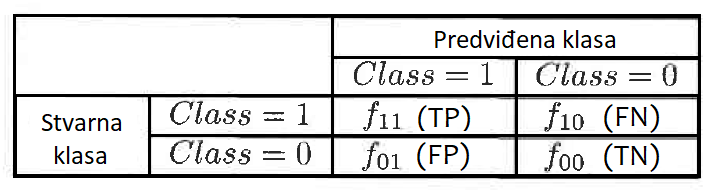
\includegraphics[width=0.60\textwidth]{matrica_konfuzije}
  \caption{Matrica konfuzije za problem binarne klasifikacije}
  \label{fig:matrkonf}
\end{figure}

 Za poređenje većeg broja modela bilo bi jednostavnije da su vrednosti matrice konfuzije predstavljene jednim brojem. U tu svrhu se mogu koristiti tačnost (eng.~accuracy)  i stopa (odnos) greške (eng.~error rate). \textit{Tačnost} je broj tačnih predviđanja podeljen ukupnim brojem predviđanja. \textit{Odnos greške} je broj pogrešnih predviđanja podeljen ukupnim brojem predviđanja. Većina algoritama treba da ostvari najveću tačnost (ili analogno najmanju stopu (odnos) greške) \cite{mitic}.

$$ \textit{Tačnost} = \frac{f_{11}+f_{00}}{f_{11}+f_{10}+f_{01}+f_{00}} $$

$$ \textit{Odnos greške} = \frac{f_{10}+f_{01}}{f_{11}+f_{10}+f_{01}+f_{00}} $$

U situacijama kada su klase nejednako zastupljene tačnost nije mera koja odgovara podacima jer svaku klasu tretira kao jednako važnu. Za problem binarne klasifikacije ređe zastupljena klasa često nosi naziv pozitivna klasa, a zastupljenija klasa nosi naziv negativna klasa. Slika \ref{fig:matrkonf2} prikazuje matricu konfuzije koja sumira broj dobro i loše klasifikovanih objekata pri čemu vrednosti matrice imaju sledeće značenje \cite{mitic}:

\begin{figure}[!ht]
  \centering
  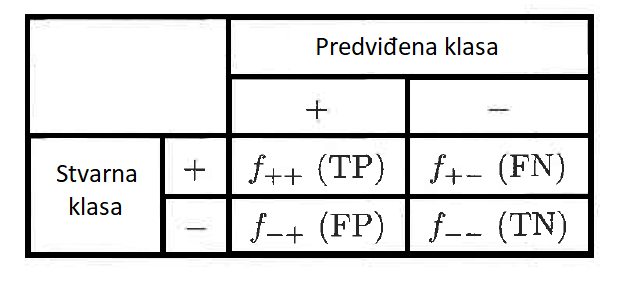
\includegraphics[width=0.60\textwidth]{matrica_konfuzije2}
  \caption{Matrica konfuzije za problem binarne klasifikacije kada dve klase nisu podjednako bitne}
  \label{fig:matrkonf2}
\end{figure}

\textit{Stvarno pozitivni (TP - true positive)} ili $f_{++}$ je broj objekata koji pripadaju pozitivnoj klasi a dodeljena im je pozitivna klasa.

\textit{Lažno negativni (FP - false negative)} ili $f_{+-}$ je broj objekata koji pripadaju pozitivnoj klasi a dodeljena im je negativna klasa.

\textit{Lažno pozitivni (FP - false positive)} ili $f_{-+}$ je broj objekata koji pripadaju negativnoj klasi a dodeljena im je pozitivna klasa.

\textit{Stvarno negativni (TN - true negative)} ili $f_{--}$ je broj objekata koji pripadaju negativnoj klasi a dodeljena im je negativna klasa.

Metrike koje se sa dosta uspeha koriste kada je potrebno otkriti jednu od klasa su preciznost i odziv. \textit{Preciznost} (eng.~precision) je procenat stvarno pozitivnih objekata među objektima koji su klasifikovani kao pozitivni. Veća preciznost takođe znači da postoji manji broj lažno pozitivnih objekata. \textit{Odziv} (eng.~recall) predstavlja procenat pozitivnih objekata koji su ispravno klasifikovani. Visok odziv znači da postoji mali broj lažno negativnih objekata. Preciznost i odziv se mogu sumirati u metriku koja se zove $F_1\ mera$ (eng.~$F_1$ measure)  \cite{mitic}.

$$ \textit{Preciznost} = \frac{TP}{TP+FP} $$

$$ \textit{Odziv} = \frac{TP}{TP+FN} $$ 

$$ F_1\ mera = \frac{2TP}{2TP+FP+FN}$$

% \subsection{ROC kriva}

%ROC (eng.~Receiver Operating Characteristic) kriva služi za grafički prikaz odnosa stvarno pozitivnih i lažno pozitivnih objekata matrice konfuzije

\subsection{Upoznavanje sa podacima}  \label{upoznavanje}

\textit{Preprocesiranje podataka} (eng.~data preprocessing) je široka oblast koja obuhvata različite tehnike i strategije koje se koriste zarad dobijanja podataka pogodnijih za rad. Te tehnike i strategije spadaju ili u izbor objekata i atributa za analizu ili u kreiranje novih atributa/menjanje postojećih atributa i ne postoji generalno pravilo kojim redom će se one primenjivati. Na izbor tehnika i strategija utiče priroda podataka sa kojima se radi \cite{mitic}. 

Upoznavanje sa podacima je neizostavan korak u procesu dobijanja kvalitetnog klasifikacionog modela. Od prirode podataka zavisi koji koji algoritmi se mogu koristiti za dobijanje modela, kao i kakve transformacije podataka su potrebne ili neophodne da bi dobijeni modeli bili verodostojni.
Zbog toga je najpre potreno upoznati se sa raspoloživim podacima. Broj podataka i atributi su poznati iz dela \ref{kor_podaci}. Jedna od prvih provera je da li postoje podaci sa nedostajućim vrednostima. Takvih podataka nema u korišćenom korpusu, tako da neće biti više reči na ovu temu. U slučaju da postoje podaci sa nedostajućim vrednostima, mogu se tretirati na neki od načina opisanih u \cite{mitic}. Takođe je potrebno proveriti raspodelu klasa među podacima. Na slici \ref{fig:raspodela} vidi se da su podaci prilično neravnomerno raspoređeni. Podaci koji nemaju grešku su daleko zastupljeniji od podataka koji imaju grešku. Od 10878 podataka, čak 8776 podataka su podaci koji imaju grešku, a 2102 nema grešku i ovo može predstavljati problem. Ovakva pojava predstavlja problem neizbalansiranih klasa. Modeli trenirani nad podacima koji imaju ovako velike razlike u raspodeli klasa mogu davati pristrasne rezultate tj. težiti da novim instancama dodele zastupljeniju klasu (u ovom slučaju je to klasa programa koji nemaju greške). Kako su podaci od interesa programi kod kojih greška postoji takvo ponašanje modela je posebno nedopustivo. Problem neizbalansiranih klasa se može rešiti na nekoliko načina. U ovom radu problem je rešen dodavanjem novih instanci (eng.~oversampling) što je detaljnije opisano u delu \ref{oversampling}. Postoji nekoliko koraka urađenih pre dodavanja novih instanci kojima je potrebno posvetiti više pažnje.  

\begin{figure}[!ht]
  \centering
  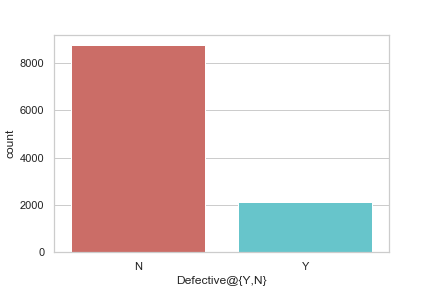
\includegraphics[width=0.80\textwidth]{raspodela.png}
  \caption{Raspodela objekata prema atributu klase}
  \label{fig:raspodela}
\end{figure}
	 
\subsection{Transformacija atributa}

Termin \textit{transformacija atributa} označava transformaciju koja se primenjuje na sve vrednosti atributa. To znači da će vrednost atributa svakog objekta biti transformisana. Postoje različiti tipovi transformacija, a koji tip će biti korišćen zavisi od prirode podataka. U nekim situacijama je dovoljno primeniti jednostavnu matematičku funkciju na vrednosti atributa $x$ (npr. $x^k$, $\log x$, $\sqrt{x}$, $\left| x \right|$, ...) . U nekim drugim situacijama potrebno je izvršiti normalizaciju ili standardizaciju \footnote{Neke literature ne prave razliku između ova dva termina. Međutim, paket scikit-learn razlikuje normalizaciju i standardizaciju pa će stoga biti razlikovane i u ovoj tezi. Dodatno, u tezi se za transformaciju podataka koristi samo standardizacija pa će ona biti detaljnije objašnjena.}. Cilj normalizacije i standardizacije je da transformacijama skup vrednosti dobije određena svojstva \cite{mitic}.  

\textit{Standardizacija} je tehnika transformisanja atributa na taj način što se od svake vrednosti atributa oduzima njegova sredina, a zatim se dobijena vrednost deli standardnom devijacijom atributa. Na ovaj način se dobijaju nove vrednosti atributa, a sam atribut će imati sredinu 0 i standardnu devijaciju 1. Standardizacija je često neophodna za veliki broj algoritama mašinskog učenja paketa scikit-learn. U slučaju da atributi nemaju raspodelu podataka sličnu normalnoj ili Gausovoj algoritmi mašinskog učenja mogu proizvesti pogrešne rezultate. Standardizacija je takođe često neophodna ako se veći broj promenljivih međusobno kombinuju. Standardizacijom se sprečava uticaj promenljive sa visokim vrednostima atributa na rezultat izračunavanja. Jednostavan ali slikovit primer kada treba primeniti standardizaciju je situacija u kojoj treba porediti dve osobe na osnovu godina i plate. Razlike u platama mogu biti veće od razlika u godinama zato što se njihovi opsezi vrednosti dosta razlikuju (godine su broj manji od 100, a plate se mere u desetinama ili stotinama hiljada). U takvoj situaciji, ukoliko se ove razlike ne uzmu u obzir, na rezultat poređenja će najviše uticati razlike u platama (Euklidsko rastojanje je jedna od metrika kod koje se moraju uzeti u obzir razlike u opsezima atributa) \cite{ sklearn_preprocessing, mlm2, mitic}. 

Na slici \ref{fig:atr_opsezi} vidi se da se opsezi vrednosti atributa dosta razlikuju. Zbog toga je potrebno izvršiti standardizaciju podataka kako atributi sa visokim vrednostima ne bi previše uticali na rezultat klasifikacije. 

\begin{figure}[!ht]
  \centering
  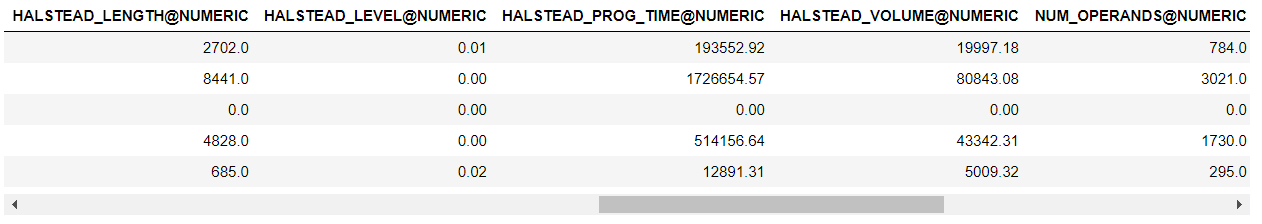
\includegraphics[width=1\textwidth]{atr_opsezi.png}
  \caption{Opsezi vrednosti za neke od atributa}
  \label{fig:atr_opsezi}
\end{figure}

\subsection{Treniranje modela klasifikacije i njihove ocene}

Nakon osnovnog upoznavanja sa podacima i urađene standardizacije mogu se konstruisati inicijalni modeli klasifikacije za svaki algoritam. Rad sa klasifikacionim modelima u Python-u je prilično jednostavan i gruba skica bi se sastojala od četiri koraka \cite{scikit-learn}:

Na početku je potrebno skup podataka podeliti na skup za trening i skup za testiranje (npr. u odnosu 60:40) da bi kasnije bilo moguće proceniti kvalitet modela. Za podelu skupa podataka dovoljno je pozvati metod \textit{train\_test\_split} koji pripada modulu \textit{model\_selection} u okviru paketa \textit{sklearn} (scikit-learn). Treba napomenuti da je podela skupa podataka na skupove za treniranje i testiranje (kao i unakrsna validacija koja je takođe korišćena u tezi) samo način da se izvrši procena kvaliteta dobijenog modela (kao što je opisano u delu \ref{evaluacija}). Konačni model koji će se koristiti za dodeljivanje klasa nepoznatim podacima treba da se obuči nad celokupnim skupom raspoloživih podataka \cite{mladen}.

\begin{lstlisting}[language=Python, basicstyle=\tiny]
	from sklearn.model_selection import train_test_split
	X_train, X_test, y_train, y_test = 
		train_test_split(X, y, test_size=0.4, random_state=42)
\end{lstlisting}

Zatim se iz odgovarajućeg paketa učitava i kreira klasifikacioni model \footnote{U ovoj tezi se prilikom kreiranja klasifikatora zasnovanih na algoritmu k najbližih suseda za vrednosti k uzimaju 3 i 15 (u zavisnosti od situacije). Do ovih vrednosti se došlo konstruisanjem algoritama za vrednosti k = 1..25 i poređenjem tačnosti dobijenih klasifikatora. Izabrane vrednosti k su one za koje su dobijeni modeli imali najveću ili skoro najveću tačnost, a da su neparan broj.}. 
\begin{lstlisting}[language=Python, basicstyle=\tiny]
	# from sklearn.neighbors import KNeighborsClassifier
	# clf = KNeighborsClassifier(n_neighbors=15)
	# from sklearn.linear_model import LogisticRegression
	# clf = LogisticRegression(random_state=0)
	from sklearn.ensemble import RandomForestClassifier
	clf = RandomForestClassifier(n_jobs=2, random_state=0)
\end{lstlisting}

Klasifikator uči model na osnovu trening podataka pomoću metoda \textit{fit}. 
\begin{lstlisting}[language=Python, basicstyle=\tiny]
	clf.fit(X_train, np.ravel(y_train))
\end{lstlisting}

Konačno, metodom $predict$ se model primeni na test podatke.
\begin{lstlisting}[language=Python, basicstyle=\tiny]
	y_pred = clf.predict(X_test)
\end{lstlisting}

Na slici \ref{fig:confmatr} mogu se videti tačnosti i matrice konfuzije za svaki od tri klasifikaciona modela. Na prvi pogled se vidi da sva tri algoritma daju modele sličnih tačnosti: 0,805, 0,810 i 0,810 (10-slojnom unakrsnom validacijom su dobijene tačnosti modela 0,776, 0,797 i 0,775). Pošto je tačnost modela broj u opsegu [0-1] za sve modele bi se moglo reći da su prihvatljivi. Tačnost modela može često da zavara i sama po sebi nije dovoljna da bi se donela presuda o kvalitetu modela pa je zato potrebno detaljnije analizirati dobijene rezultate. Dobijeni modeli sadrže relativno veliki broj (oko 700) lažno negativnih predviđanja. Ovakvi rezultati pokazuju da dobijeni modeli zapravo nisu dobri. Zadatak modela je otkrivanje programa koji imaju grešku, a u praksi će velikom broju programa sa greškom biti pogrešno dodeljena klasa programa bez greške. Primećeno ponašanje modela je posledica naizbalansiranosti klasa (kao što je napomenuto u delu \ref{upoznavanje}). 

\begin{figure}[!ht]
    \centering
    \begin{subfigure}[b]{0.45\textwidth}
        \centering
        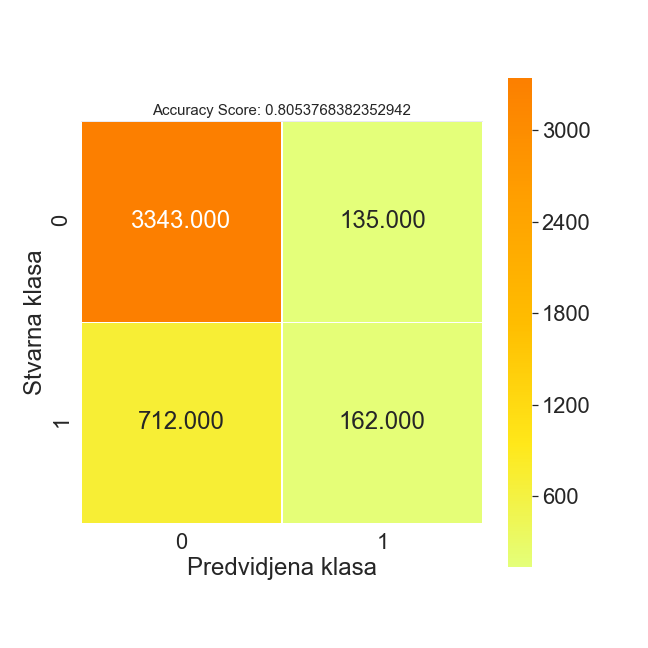
\includegraphics[width=\textwidth]{KNN_basic_data_confussion_matrix}
        \caption{k najbližih suseda}
        \label{fig:knear}
    \end{subfigure}
    \begin{subfigure}[b]{0.45\textwidth}
        \centering
        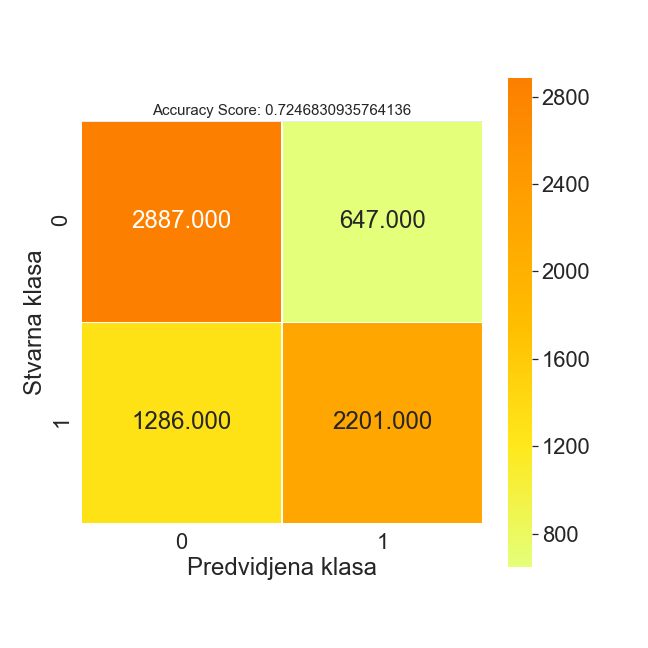
\includegraphics[width=\textwidth]{LR_basic_data_confussion_matrix}
        \caption{logistička regresija}
        \label{fig:logreg}
    \end{subfigure}
    \\
    \begin{subfigure}[b]{0.45\textwidth}
        \centering
        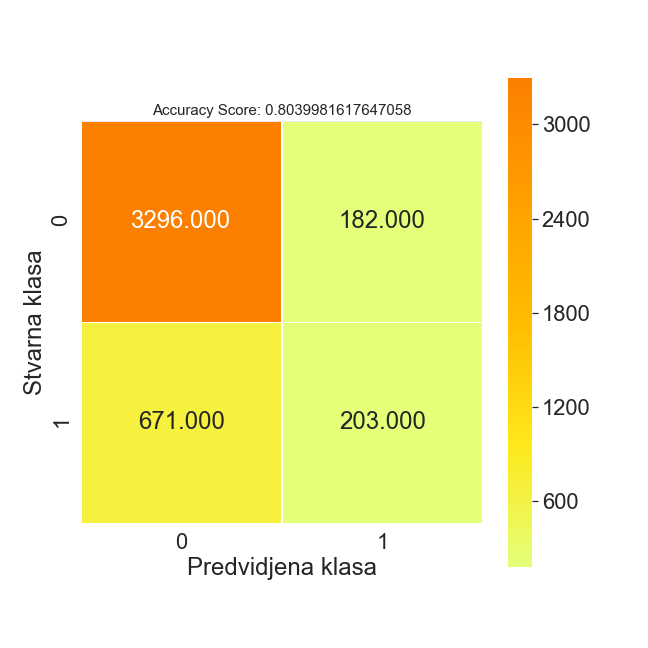
\includegraphics[width=\textwidth]{RF_basic_data_confussion_matrix}
        \caption{slučajne šume}
        \label{fig:randfor}
    \end{subfigure}
    \caption{Matrice konfuzije za klasifikatore zasnovane na različitim algoritmima}
    \label{fig:confmatr}
\end{figure}

Informacije na osnovu kojih se može izvršiti nešto detaljnija analiza modela prikazane su na slici \ref{fig:dodatno1} i one su dobijene kao rezultat poziva metoda \textit{classification\_report}. Ove se može videti da je preciznost predviđanja u slučaju programa čija je klasa 1 (tj. programa koji sadrže grešku) u proseku oko 60\% čime je potvrđeno ranije uočeno nepoželjno ponašanje modela. 

\begin{figure}[!ht]
    \centering
    \begin{subfigure}[b]{0.45\textwidth}
        \centering
        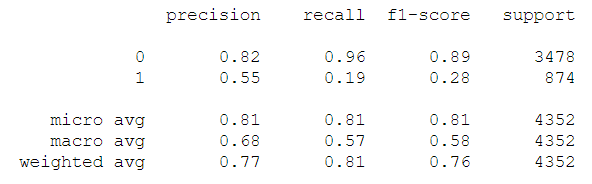
\includegraphics[width=\textwidth]{knn1}
        \caption{k najbližih suseda}
        \label{fig:kn1}
    \end{subfigure}
    \begin{subfigure}[b]{0.45\textwidth}
        \centering
        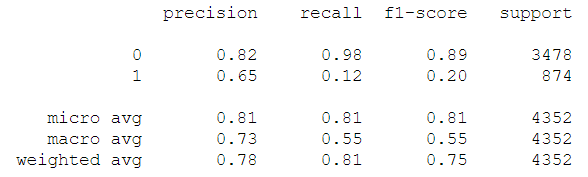
\includegraphics[width=\textwidth]{logreg1}
        \caption{logistička regresija}
        \label{fig:logreg1}
    \end{subfigure}
    \\
    \begin{subfigure}[b]{0.45\textwidth}
        \centering
        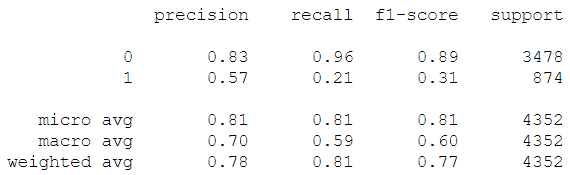
\includegraphics[width=\textwidth]{randfor1}
        \caption{slučajne šume}
        \label{fig:randfor1}
    \end{subfigure}
    \caption{Preciznost, odziv, f1-mera i podrška za klasifikatore zasnovane na različitim algoritmima}
    \label{fig:dodatno1}
\end{figure}


\subsection{Dodavanje novih instanci - Oversampling} \label{oversampling}
% uzorkovanje - manipulisanje instancama/uzorcima

Jedan od načina rešavanja problema neizbalansiranih klasa je \textit{uzorkovanje} (eng.~sampling) sa ciljem modifikovanja raspodele instanci. Posledica ovakve modifikacije raspodele je da ređe zastupljena klasa postaje reprezentativna u skupu trening podataka tj. da se poveća njen uticaj na klasifikacioni model. Uzorkovanje obuhvata dodavanje novih instanci (eng.~oversampling), uklanjanje postojećih instanci (eng.~undersampling) i kombinaciju prethodne dve tehnike \cite{mitic, aggarwal}. 

\textit{Uklanjanje postojećih instanci} je tehnika transformisanja trening skupa uklanjanjem nekih od podataka koji pripadaju zastupljenijoj klasi originalnog skupa podataka za trening. Ova tehnika nije korišćena u tezi jer bi se njenom primenom količina podataka raspoloživa za obučavanje klasifikacionih modela smanjila sa 10878 na svega 4204.
\textit{Dodavanje novih instanci} je tehnika transformisanja trening skupa dodavanjem novih podataka nastalih na osnovu nekih od podataka koji pripadaju manje zastupljenoj klasi originalnog skupa podataka za trening. U Python-u je dodavanje novih instanci podržano u okviru paketa \textit{imbalanced-learn} koji pruža mogućnost korišćenja četiri metoda dodavanja novih instanci - slučajno dodavanje (RandomOverSampler), SMOTE, SMOTE-NC i ADASYN. RandomOverSampler kreira nove uzorke na osnovu postojećih podataka metodom slučajnog izbora sa zamenom. ADASYIN i SMOTE nove uzorke kreiraju interpolacijom. Fokus ADASYIN-a je na kreiranju podataka koji se nalaze u blizini originalnih podataka pogrešno klasifikovanih od strane algoritma k najbližih suseda. Sa druge strane, SMOTE podjednako tretira sve podatke (bez obzira na to kako su klasifikovani algoritmom k najbližih suseda). SMOTE-NC služi za rad sa skupovima podataka koji sadrže neprekidne i kategoričke atribute. U ovoj tezi korišćen je metod SMOTE \cite{imblearn, mitic}.
% za smote ima dodatno u data mining the textbook, aggarwal

\begin{lstlisting}[language=Python, basicstyle=\tiny]
	from imblearn.over_sampling import SMOTE
	X_resampled, y_resampled = SMOTE(kind="svm").fit_sample(X, y)
\end{lstlisting}

Nakon dodavanja novih podataka potrebno je ponovo proći postupak obučavanja modela. Odgovarajuće matrice konfuzije prikazane su na slici \ref{fig:confmatrovers}. Procenjene tačnosti modela na osnovu podele skupa podataka na trening i test skup iznose 0,814, 0,711 i 0,859, a na osnovu 10-slojne unakrsne validacije 0,811, 0,642 i 0,834. Ono što iskače u prvi plan je vidno lošija tačnost modela zasnovanog na algoritmu logističke regresije što se posebno može primetiti evaluacijom pomoću tehnike unakrsne validacije. Takođe, modeli zasnovani na algoritmima k najbližih suseda i slučajne šume deluju stabilnije prilikom obe vrste evaluacije. 

\begin{figure}[!ht]
    \centering
    \begin{subfigure}[b]{0.45\textwidth}
        \centering
        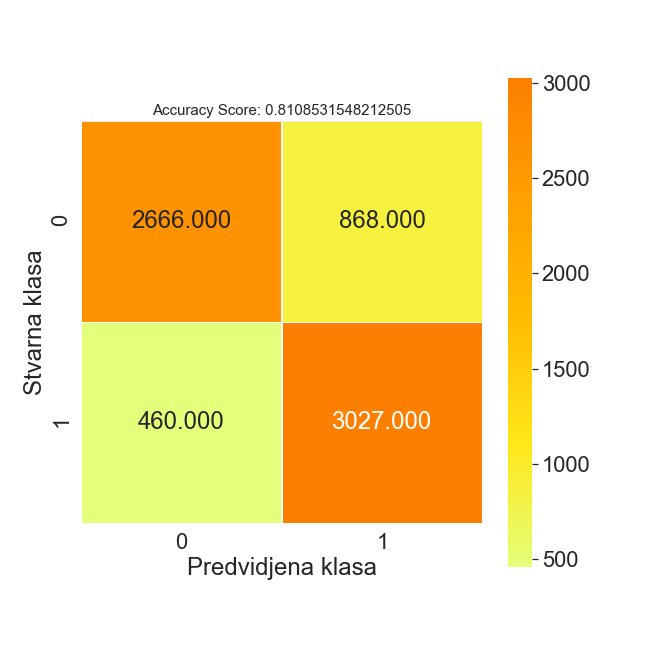
\includegraphics[width=\textwidth]{KNN_oversampled_confussion_matrix}
        \caption{k najbližih suseda}
        \label{fig:knear2}
    \end{subfigure}
    \begin{subfigure}[b]{0.45\textwidth}
        \centering
        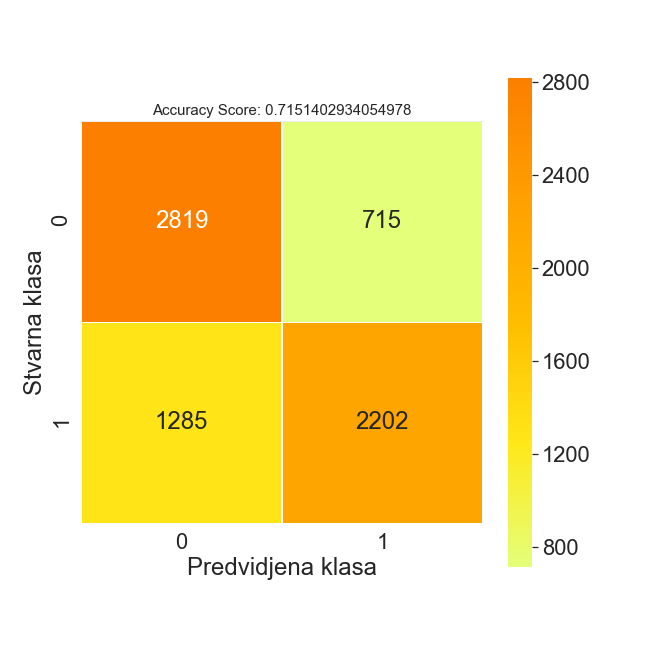
\includegraphics[width=\textwidth]{LR_oversampled_confussion_matrix}
        \caption{logistička regresija}
        \label{fig:logreg2}
    \end{subfigure}
    \\
    \begin{subfigure}[b]{0.45\textwidth}
        \centering
        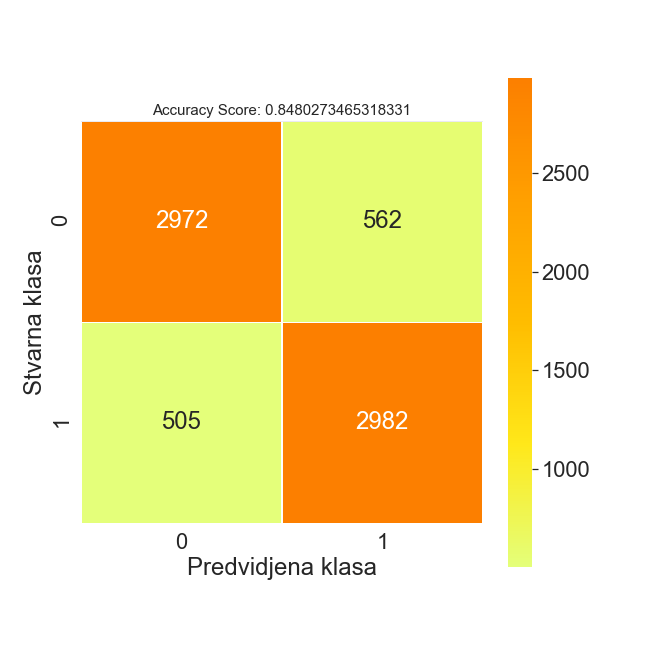
\includegraphics[width=\textwidth]{RF_oversampled_confussion_matrix}
        \caption{slučajne šume}
        \label{fig:randfor2}
    \end{subfigure}
    \caption{Matrice konfuzije za klasifikatore zasnovane na različitim algoritmima nakon dodavanja novih podataka}
    \label{fig:confmatrovers}
\end{figure}

Dodatne informacije o modelima prikazane su na slici \ref{fig:dodatno2}. Ponovo je interesantna preciznost, ovaj put modela \ref{fig:kn3} i \ref{fig:randfor3}. U slučaju klase 0 preciznost iznosi 0,85 za oba algoritma, a u slučaju klase 1 bolje rezultate daje model zasnovan na algoritmu slučajne šume (0,87 naspram 0,78). Zbog toga što je klasa od interesa klasa 1 (programi koji sadrže grešku) trenutno najbolji model je model zasnovan na algoritmu slučajne šume. Osim toga, na osnovu dobijenih rezultata deluje da model zasnovan na algoritmu logističke regresije ne uspeva dobro da prikaže prirodu podataka. Još jednu transformaciju je potrebno uraditi pre konačne presude.

\begin{figure}[!ht]
    \centering
    \begin{subfigure}[b]{0.45\textwidth}
        \centering
        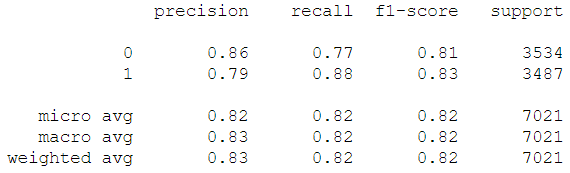
\includegraphics[width=\textwidth]{knn2}
        \caption{k najbližih suseda}
        \label{fig:kn3}
    \end{subfigure}
    \begin{subfigure}[b]{0.45\textwidth}
        \centering
        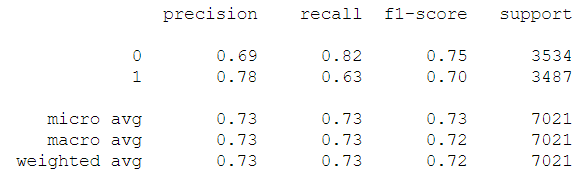
\includegraphics[width=\textwidth]{logreg2}
        \caption{logistička regresija}
        \label{fig:logreg3}
    \end{subfigure}
    \\
    \begin{subfigure}[b]{0.45\textwidth}
        \centering
        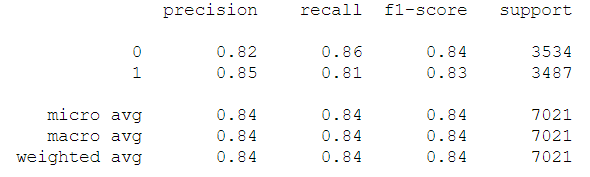
\includegraphics[width=\textwidth]{randfor2}
        \caption{slučajne šume}
        \label{fig:randfor3}
    \end{subfigure}
    \caption{Preciznost, odziv, f1-mera i podrška za klasifikatore zasnovane na različitim algoritmima nakon dodavanja novih podataka}
    \label{fig:dodatno2}
\end{figure}

\subsection{Izbor atributa}

Skupovi podataka mogu da sadrže podatke sa velikim brojem atributa tj. podatke koji imaju visoku dimenzionalnost. Jedan takav primer je matrica terma dokumenata (eng.~document term matrix) čiji su redovi dokumenti, kolone su termi odnosno reči, a u preseku redova i kolona se nalaze vrednosti koje predstavljaju broj pojavljivanja reči u dokumentu. Ove matrice potencijalno mogu imati hiljade ili desetine hiljada atributa \cite{mitic}. 

Postoje brojne prednosti smanjenja dimenzionalnosti: algoritam mašinskog učenja zahteva manje vremena i memorije, algoritam mašinskog učenja može pružati bolje performanse u slučaju manjih dimenzija jer se smanjenjem dimenzije eliminišu nebitni atributi i umanjuje šum, a takođe se i rešava problem prokletstva dimenzionalnosti \footnote{Prokletstvo dimenzionalnosti (eng.~the curse of dimensionality) je situacija u kojoj analiza podataka postaje sve teža sa porastom dimenzionalnosti.}, dobijeni model je lakši za tumačenje ako je manji broj atributa uključen i vizualizacija podataka je olakšana ako postoji manji broj atributa \cite{mitic, UMLFTA}.

Smanjenje dimenzionalnosti često se odnosi na tehnike koje do smanjenja vode pravljenjem novih atributa kombinovanjem postojećih. Do smanjenja dimenzionalnosti može se doći i tako što novi atributi predstavljaju podskup postojećih. Ova tehnika zove se \textit{izbor podskupa atributa} (eng.~feature subset selection) ili kraće \textit{izbor atributa} (eng.~feature selection). Iako deluje da bi se izborom atributa mogle izgubiti bitne informacije ovo nije slučaj ukoliko postoje nevažni i redundantni atributi. Redundantni atributi dupliraju informaciju koja je već postojana u nekom drugom atributu (npr. cena atrikla i porez), dok nevažni atributi ne sadrže informacije od značaja (npr. indeksi studenata prilikom predviđanja ocene na ispitu) \cite{mitic}. 

Idealan pristup izboru atributa je isprobavanje svih mogućih kombinacija atributa za ulaz u algoritam mašinskog učenja. U praksi ovo nije izvodljivo jer je broj podskupova za $n$ atributa jednak $2^n$. Postoje tri često korišćene grupe pristupa za izbor atributa: 1) ugrađeni pristupi (eng.~embedded approaches) - izbor atributa dešava se prilikom izvršavanja algoritma mašinskog učenja tj. prilikom obučavanja klasifikacionog modela kada algoritam bira koje atribute da zadrži a koje da zanemari, 2) pristupi koji koriste filtere (eng.~filter approaches) - izbor atributa vrši se pre pokretanja algoritma mašinskog učenja i nezavisno od samog zadatka istraživanja podataka i 3) pristupi koji koriste omotače (eng.~wrapper approaches) - za izbor atributa se, kao crna kutija, koristi neki algoritam mašinskog učenja \cite{mitic, UMLFTA, aggarwal}.

Scikit-learn pruža nekoliko načina za izbor atributa, a u ovoj tezi je korišćen izbor atributa koji se zasniva na značaju atributa. Model \textit{ExtraTreesClassifier} konstuiše veći broj stabala odlučivanja na različitim podskupovima originalnog skupa podataka, a zatim pomoću tehnike uprosečavanja pokušava da poboljša tačnost predviđanja i da kontroliše preprilagođavanje. Po završetku ovog posla pomoću metoda \textit{feature\_importances\_} dobijaju se vrednosti koje odgovaraju značaju atributa \cite{scikit-learn}. 

\begin{figure}[!ht]
  \centering
  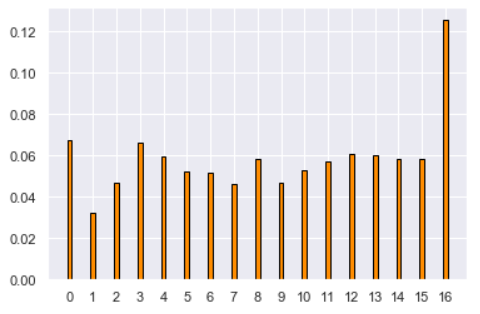
\includegraphics[width=0.60\textwidth]{izbor_atributa}
  \caption{Značaj atributa}
  \label{fig:znacaj}
\end{figure}

Na slici \ref{fig:znacaj} prikazan je rezultat poziva metoda \textit{feature\_importances\_}. na $x$ osi se nalaze indeksi atributa, a na $y$ osi značaj atributa. U cilju poboljšanja tačnosti i/ili brzine modela na osnovu značaja atributa biće sačuvano 10 najznačajnijih atributa a ostali će biti odbačeni. Tih 10 najznačajnijih atributa, u rastućem poretku su: \textit{HALSTEAD\_VOLUME, 
HALSTEAD\_LENGTH, 
NUM\_OPERATORS, \\
NUM\_UNIQUE\_OPERATORS, 
NUM\_UNIQUE\_OPERANDS, \\HALSTEAD\_CONTENT, 
NUM\_OPERANDS, LOC\_EXECUTABLE, \\
LOC\_BLANK i LOC\_TOTAL}.

\subsection{Konačni izgled modela}

Slika \ref{fig:confmatroversfeatsel} pokazuje da se izborom atributa dobijaju modeli nešto lošije tačnosti u odnosu na modele obučavane nad podacima na kojima nije vršen izbor atributa. To potvrđuju i rezultati 10-slojne unakrsne validacije 0,785, 0,567 i 0,829. Slika \ref{fig:dodatno3} pokazuje da su i preciznosti modela takođe lošije nakon izbora atributa. Najmanja razlika u preciznosti (a takođe i u tačnosti modela) je kod modela zasnovanog na algoritmu slučajnih šuma. 

Na osnovu do sada viđenog može se zaključiti da je model koji najviše odgovara podacima model koji je zasnovan na algoritmu slučajnih šuma. Izborom atributa nisu dobijeni bolji rezultati u smislu tačnosti modela, ali rezultati nisu ni mnogo lošiji u odnosu na model dobijen nad podacima kod kojih nije rađen izbor atributa. Zbog toga, u nadi da će to dovesti do uštede u vremenu obučavanja, prilikom obučavanja konačnog modela biće primenjen izbor atributa. Konačan model koji će se koristiti za klasifikaciju nepoznatih programa biće model zasnovan na algoritmu slučajnih šuma, obučavaće se nad svim raspoloživim podacima pri čemu će nad podacima biti urađen izbor atributa.

\begin{figure}[!ht]
    \centering
    \begin{subfigure}[b]{0.45\textwidth}
        \centering
        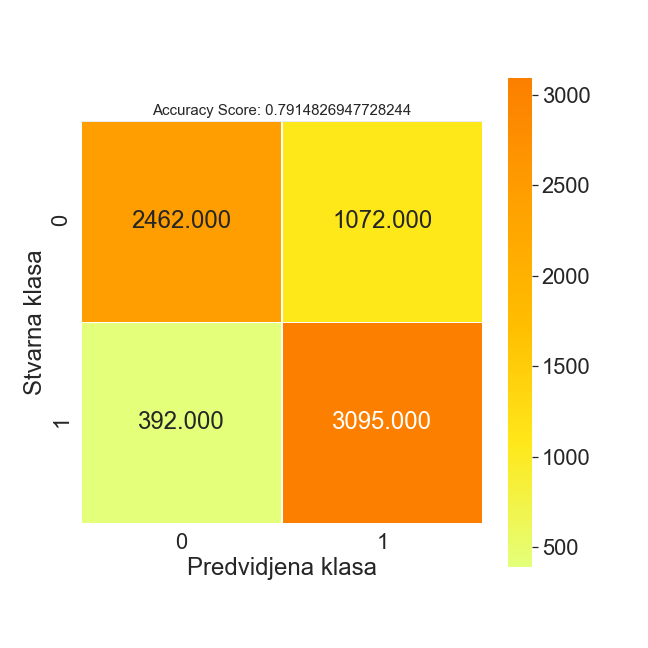
\includegraphics[width=\textwidth]{KNN_feature_selection_oversampled_confussion_matrix}
        \caption{k najbližih suseda}
        \label{fig:knear4}
    \end{subfigure}
    \begin{subfigure}[b]{0.45\textwidth}
        \centering
        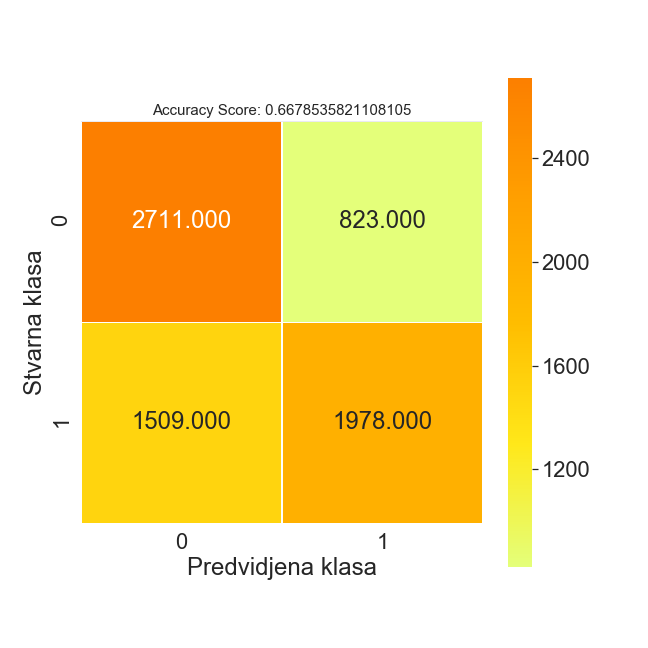
\includegraphics[width=\textwidth]{LR_feature_selection_oversampling_confussion_matrix}
        \caption{logistička regresija}
        \label{fig:logreg4}
    \end{subfigure}
    \\
    \begin{subfigure}[b]{0.45\textwidth}
        \centering
        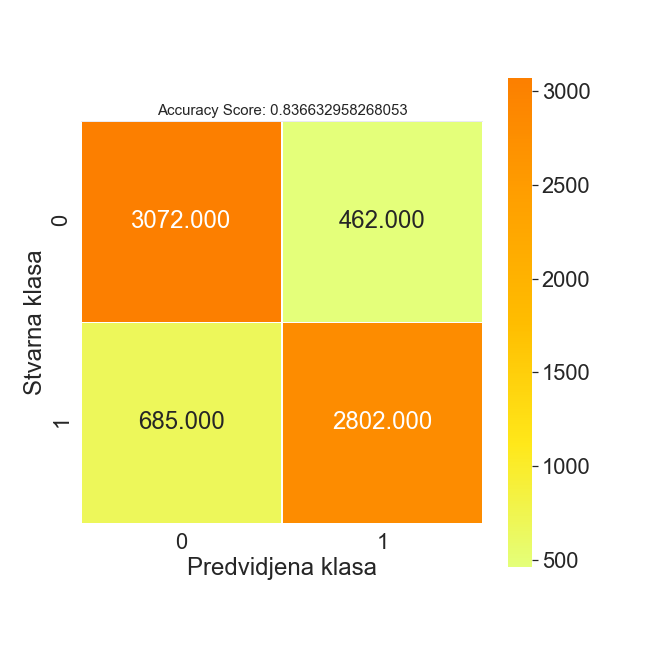
\includegraphics[width=\textwidth]{RF_feature_selection_oversampled_confussion_matrix}
        \caption{slučajne šume}
        \label{fig:randfor4}
    \end{subfigure}
    \caption{Matrice konfuzije za klasifikatore zasnovane na različitim algoritmima nakon dodavanja novih podataka i izbora atributa}
    \label{fig:confmatroversfeatsel}
\end{figure}

\begin{figure}[!ht]
    \centering
    \begin{subfigure}[b]{0.45\textwidth}
        \centering
        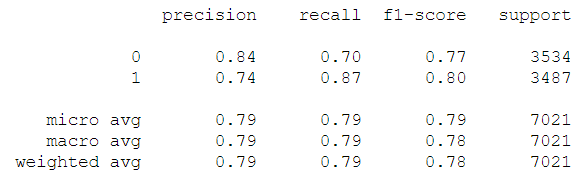
\includegraphics[width=\textwidth]{knn_final}
        \caption{k najbližih suseda}
        \label{fig:kn_final}
    \end{subfigure}
    \begin{subfigure}[b]{0.45\textwidth}
        \centering
        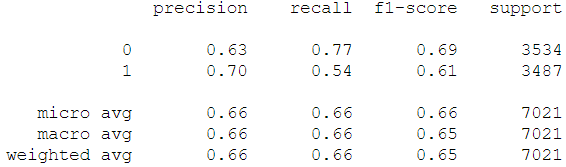
\includegraphics[width=\textwidth]{logreg_final}
        \caption{logistička regresija}
        \label{fig:logreg_final}
    \end{subfigure}
    \\
    \begin{subfigure}[b]{0.45\textwidth}
        \centering
        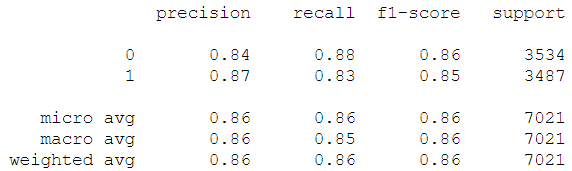
\includegraphics[width=\textwidth]{randfor_final}
        \caption{slučajne šume}
        \label{fig:randfor_final}
    \end{subfigure}
    \caption{Preciznost, odziv, f1-mera i podrška za klasifikatore zasnovane na različitim algoritmima nakon dodavanja novih podataka i izbora atributa}
    \label{fig:dodatno3}
\end{figure}

% 
% ROC krive?

\section{Program koji iz C koda dobija atribute}

Ulazi modela klasifikacije su atributi C programa. Da bi se za proizvoljan program mogla raditi klasifikacija neophodno je njegov izvorni k\^od prevesti u atribute. U tu svrhu implementiran je program koji na osnovu izvornog koda programa napisanog u C-u dobija atribute opisane u delu \ref{kor_podaci}. Ovaj program napisan je u jeziku Python i većim delom se zasniva na biblioteci \textit{pycparser}. Pycparser je parser programskog jezika C implementiran u Python-u. Detalji o modulu mogu se pronaći na linku: \url{https://github.com/eliben/pycparser} odakle se može izvršiti i njegovo preuzimanje. Korisne informacije se mogu naći i na veb strani autorke: \url{https://eli.thegreenplace.net/}.

Kako se atributi sa kojima se radi mogu podeliti u dve grupe (atributi koji se odnose na Halstedove metrike i atributi koji se odnose na linije koda) tako se postupak izračunavanja atributa na osnovu C koda može opisati u dva koraka. 

\begin{description}
\item[Izračunavanje atributa koji se odnose na Halstedove metrike]

Halstedove metrike se koriste da bi se izmerili veličina softverskog proizvoda, kao i cena i napor potrebni za njegov razvoj. Ove metrike se zasnivaju na broju operatora i broju operanada izvornog koda. Preciznije, u pitanju su četiri atributa koda: broj jedinstvenih operatora, broj jedinstvenih operanada, ukupan broj operatora i ukupan broj operanada. Smernice za izračunavanje operanada i operatora za programski jezik C izgledaju ovako \cite{halstead}:
\begin{description}
\item[Operandi]
	\begin{enumerate}[(a)]
		\item[]
		\item Identifikatori - svi identifikatori koji ne spadaju u ključne reči
		\item Imena tipova - int, float, char, double, long, short, signed, unsigned, void, ... 
		\item Konstante - bilo da im je sadržaj karakter, string ili broj
	\end{enumerate}

\item[Operatori]
	\begin{enumerate}[(a)]
		\item[]
		\item Specifikatori koji se odnose na skladišta - auto, extern, register, static, typedef
		\item Kvalifikatori tipova - const, final, volatile
		\item Razne rezervisane reči kao što su: break, case, continue, default, do, if, else, enum, for, goto, if, new, return, sizeof, struct, switch, union, while. 
		\item Operatori - svi operatori programskog jezika C
% ! != \% \%= \& \&\& || \&= ( ) \{ \} [ ] * *= + ++ += , - -- -= -> . \/ \/= : :: < << <<= <= = == > >= >> >>= ? \^{} \^{}= | |= ~ ; =\& \# \#\# '' ""
	\end{enumerate}
\end{description}
Potrebno je napomenuti i neke specijalne slučajeve \cite{halstead}: 
\begin{enumerate}
	\item Par zagrada je jedan operator
	\item Jedan operator su takođe i delimiter ; kao i ternarni operator ?:
	\item Labele su operatori ako se koriste u okviru goto konstrukta
	\item Dvotačka u okviru case:, kao i par zagrada u okviru for(), if(), while(), switch() predstavljaju deo konstrukta i jedan operator 
	\item Komentari ne spadaju ni u operatore ni u operande
	\item Imena funkcija su operatori ako je u pitanju poziv funkcije. Imena funkcija u deklaraciji i definiciji nisu operatori
	\item Prethodno pravilo takođe važi i za promenljive i konstante
\end{enumerate}

Pomoću biblioteke pycparser moguće je na osnovu datih smernica prebrojati operatore i operanade. Izračunavanje atributa koji se zasnivaju na operandima i operatorima je malo složenije od jednostavnog prebrojavanja i započinje parsiranjem C koda metodom \textit{parse\_file}. Rezultat parsiranja je \textit{AST stablo}. AST stablo (eng.~Abstract Syntax Tree) je drvolika reprezentacija sintakse izvornog koda programa pogodna za analizu i manipulaciju. Dobijeno AST stablo prepoznaje 47 tipova čvorova (neki od njih su: Assignment, BinaryOp, For, If, Return, Struct, Switch, Typedef, While, ...) koji se odnose na strukturu C koda. Obilaskom AST stabla, analizom njegovih čvorova i primenom prethodno navedenih smernica na čvorove stabla zabeleženi su svi operandi i većina operatora. Operatori koji su ostali nezabeleženi su: ( ) [ ] \{ \} , ; : \# \#\# ' i ''. Ovi operatori su prebrojani regularnim izrazima zbog jednostavnosti. Po završetku prebrojavanja operatora i operanada moguće je izračunati atribute koji se na njih odnose. Nakon toga jednostavnom primenom formula iz \ref{kor_podaci} mogu se izračunati potrebne Halstedove metrike \cite{pycparser}.

\item[Izračunavanje atributa koji se odnose na linije koda]

Atributi koji se odnose na linije koda programa su računati na različite načine. Broj izvršivih linija koda LOC\_EXEC se računa prilikom obilaska čvorova AST stabla. Ukupan broj linija koda LOC\_TOTAL, kao i broj praznih linija LOC\_BLANC računaju se prebrojavanjem. Broj linija komentara LOC\_COMMENTS se računa korišćenjem regularnog izraza. Broj linija koda i komentara \\LOC\_CODE\_AND\_COMMENT se računa oduzimanjem broja praznih linija od ukupnog broja linija. 

\end{description}

\section{Primena klasifikacionog modela na izlaz programa za dobijanje atributa}

%- izlaz programa za atribute  
%- primeni se klasifikator


%---------------------

% \chapter{Eksperimentalni rezultati}

% \section{Pokretanje verifikacijskih alata i merenje performansi}

% \section{Primena izabranog modela na nove podatke}

%--------------------------
%\chapter{Primeri korišćenja klasičnih \LaTeX{} elemenata}

% Primeri citiranja
%Ovo je rečenica u kojoj se javlja citat \cite{PetrovicMikic2015}.
%Još jedan citat \cite{GuSh:243}.

% Primeri navodnika
%Isprobavamo navodnike: "Rekao je da mu se javimo sutra".

% Primer referisanja na tabelu (koja se javlja kasnije)
%U tabeli \ref{tbl:rezultati} koja sledi prikazani su rezultati eksperimenta.

% Primer kraćeg ćiriličkog teksta
%{\cir Ово је пример ћириличког текста који се јавља у латиничком документу.}
%U ovoj rečenici se javlja jedna reč na {\cir ћирилици}.

% Primer korišćenja fusnota
%Iza ove rečenice sledi fusnota.\footnote{Ovo je fusnota.}

% Primer dužeg ćirličkog teksta
%\begin{cirilica}
%  Ово је мало дужи блок текста исписан ћириличким писмом у оквиру
%  латиничког документа. Фијуче ветар у шибљу, леди пасаже и куће иза
%  њих и гунђа у оџацима.
%\end{cirilica}

% Primer korišćenja tabele
%\begin{table}
%\centering
%\caption{Rezultati}
%\label{tbl:rezultati}
%\begin{tabular}{c>{\centering}p{2cm}c}
%\toprule
%1 & 2 & 3\\\midrule
%4 & 5 & 6\\\cmidrule(rl){1-2}
%7 & 8 & 8\\
%\bottomrule
%\end{tabular}
%\end{table}

% Primer korišćenja slike
%\begin{figure}[!ht]
%  \centering
%  \label{fig:grafikon}
%  \includegraphics[width=0.5\textwidth]{graph.png}
%  \caption{Grafikon}
%\end{figure}


% Primer jednostavnije matematičke formule
%Evo i jedan primer matematičke formule: $e^{i\pi} + 1 = 0$. 

% Primer referisanja na sliku
%Na slici \ref{fig:grafikon} prikazan je jedan grafikon.

% primer kompleksnije matematičke formule
%$$
%\int_a^b f(x)\ \mathrm{d}x \ =_{def}\ \lim_{\max{\Delta x_k \rightarrow 0}} \sum_{k=1}^n f(x_k^*)\Delta x_k
%$$

% primer referisanja na poglavlja i strane poglavlja
%Više detalja biće dato u glavi \ref{chp:razrada} na strani \pageref{chp:razrada}.

% primer liste
%Možemo praviti i nabrajanja:
%\begin{enumerate}
%\item Analiza 1
%\item Linearna algebra
%\item Analitička geometrija
%\item Osnovi programiranja
%\end{enumerate}

%\pangrami

% ------------------------------------------------------------------------------





% ------------------------------------------------------------------------------

%\pangrami

%\pangrami

% ------------------------------------------------------------------------------
\chapter{Zaključak}
% ------------------------------------------------------------------------------
%\pangrami

%\pangrami

% ------------------------------------------------------------------------------
% Literatura
% ------------------------------------------------------------------------------



\literatura

% ==============================================================================
% Završni deo teze i prilozi
\backmatter
% ==============================================================================

% ------------------------------------------------------------------------------
% Biografija kandidata
\begin{biografija}
%  \textbf{Vuk Stefanović Karadžić} (\emph{Tršić,
 %   26. oktobar/6. novembar 1787. — Beč, 7. februar 1864.}) bio je
%  srpski filolog, reformator srpskog jezika, sakupljač narodnih
%  umotvorina i pisac prvog rečnika srpskog jezika.  Vuk je
%  najznačajnija ličnost srpske književnosti prve polovine XIX
%  veka. Stekao je i nekoliko počasnih mastera.  Učestvovao je u
  %Prvom srpskom ustanku kao pisar i činovnik u Negotinskoj krajini, a
%  nakon sloma ustanka preselio se u Beč, 1813. godine. Tu je upoznao
%  Jerneja Kopitara, cenzora slovenskih knjiga, na čiji je podsticaj
%  krenuo u prikupljanje srpskih narodnih pesama, reformu ćirilice i
%  borbu za uvođenje narodnog jezika u srpsku književnost. Vukovim
%  reformama u srpski jezik je uveden fonetski pravopis, a srpski jezik
  %je potisnuo slavenosrpski jezik koji je u to vreme bio jezik
%  obrazovanih ljudi. Tako se kao najvažnije godine Vukove reforme
%  ističu 1818., 1836., 1839., 1847. i 1852.
\end{biografija}
% ------------------------------------------------------------------------------

%\bibliography{rad.bib}{}
%\bibliographystyle{plain}

\end{document}